\documentclass[]{book}
\usepackage{lmodern}
\usepackage{amssymb,amsmath}
\usepackage{ifxetex,ifluatex}
\usepackage{fixltx2e} % provides \textsubscript
\ifnum 0\ifxetex 1\fi\ifluatex 1\fi=0 % if pdftex
  \usepackage[T1]{fontenc}
  \usepackage[utf8]{inputenc}
\else % if luatex or xelatex
  \ifxetex
    \usepackage{mathspec}
  \else
    \usepackage{fontspec}
  \fi
  \defaultfontfeatures{Ligatures=TeX,Scale=MatchLowercase}
\fi
% use upquote if available, for straight quotes in verbatim environments
\IfFileExists{upquote.sty}{\usepackage{upquote}}{}
% use microtype if available
\IfFileExists{microtype.sty}{%
\usepackage{microtype}
\UseMicrotypeSet[protrusion]{basicmath} % disable protrusion for tt fonts
}{}
\usepackage[margin=1in]{geometry}
\usepackage{hyperref}
\hypersetup{unicode=true,
            pdftitle={Análise de Dados Amostrais Complexos},
            pdfauthor={Djalma Pessoa e Pedro Nascimento Silva},
            pdfborder={0 0 0},
            breaklinks=true}
\urlstyle{same}  % don't use monospace font for urls
\usepackage{natbib}
\bibliographystyle{apalike}
\usepackage{color}
\usepackage{fancyvrb}
\newcommand{\VerbBar}{|}
\newcommand{\VERB}{\Verb[commandchars=\\\{\}]}
\DefineVerbatimEnvironment{Highlighting}{Verbatim}{commandchars=\\\{\}}
% Add ',fontsize=\small' for more characters per line
\usepackage{framed}
\definecolor{shadecolor}{RGB}{248,248,248}
\newenvironment{Shaded}{\begin{snugshade}}{\end{snugshade}}
\newcommand{\KeywordTok}[1]{\textcolor[rgb]{0.13,0.29,0.53}{\textbf{#1}}}
\newcommand{\DataTypeTok}[1]{\textcolor[rgb]{0.13,0.29,0.53}{#1}}
\newcommand{\DecValTok}[1]{\textcolor[rgb]{0.00,0.00,0.81}{#1}}
\newcommand{\BaseNTok}[1]{\textcolor[rgb]{0.00,0.00,0.81}{#1}}
\newcommand{\FloatTok}[1]{\textcolor[rgb]{0.00,0.00,0.81}{#1}}
\newcommand{\ConstantTok}[1]{\textcolor[rgb]{0.00,0.00,0.00}{#1}}
\newcommand{\CharTok}[1]{\textcolor[rgb]{0.31,0.60,0.02}{#1}}
\newcommand{\SpecialCharTok}[1]{\textcolor[rgb]{0.00,0.00,0.00}{#1}}
\newcommand{\StringTok}[1]{\textcolor[rgb]{0.31,0.60,0.02}{#1}}
\newcommand{\VerbatimStringTok}[1]{\textcolor[rgb]{0.31,0.60,0.02}{#1}}
\newcommand{\SpecialStringTok}[1]{\textcolor[rgb]{0.31,0.60,0.02}{#1}}
\newcommand{\ImportTok}[1]{#1}
\newcommand{\CommentTok}[1]{\textcolor[rgb]{0.56,0.35,0.01}{\textit{#1}}}
\newcommand{\DocumentationTok}[1]{\textcolor[rgb]{0.56,0.35,0.01}{\textbf{\textit{#1}}}}
\newcommand{\AnnotationTok}[1]{\textcolor[rgb]{0.56,0.35,0.01}{\textbf{\textit{#1}}}}
\newcommand{\CommentVarTok}[1]{\textcolor[rgb]{0.56,0.35,0.01}{\textbf{\textit{#1}}}}
\newcommand{\OtherTok}[1]{\textcolor[rgb]{0.56,0.35,0.01}{#1}}
\newcommand{\FunctionTok}[1]{\textcolor[rgb]{0.00,0.00,0.00}{#1}}
\newcommand{\VariableTok}[1]{\textcolor[rgb]{0.00,0.00,0.00}{#1}}
\newcommand{\ControlFlowTok}[1]{\textcolor[rgb]{0.13,0.29,0.53}{\textbf{#1}}}
\newcommand{\OperatorTok}[1]{\textcolor[rgb]{0.81,0.36,0.00}{\textbf{#1}}}
\newcommand{\BuiltInTok}[1]{#1}
\newcommand{\ExtensionTok}[1]{#1}
\newcommand{\PreprocessorTok}[1]{\textcolor[rgb]{0.56,0.35,0.01}{\textit{#1}}}
\newcommand{\AttributeTok}[1]{\textcolor[rgb]{0.77,0.63,0.00}{#1}}
\newcommand{\RegionMarkerTok}[1]{#1}
\newcommand{\InformationTok}[1]{\textcolor[rgb]{0.56,0.35,0.01}{\textbf{\textit{#1}}}}
\newcommand{\WarningTok}[1]{\textcolor[rgb]{0.56,0.35,0.01}{\textbf{\textit{#1}}}}
\newcommand{\AlertTok}[1]{\textcolor[rgb]{0.94,0.16,0.16}{#1}}
\newcommand{\ErrorTok}[1]{\textcolor[rgb]{0.64,0.00,0.00}{\textbf{#1}}}
\newcommand{\NormalTok}[1]{#1}
\usepackage{longtable,booktabs}
\usepackage{graphicx,grffile}
\makeatletter
\def\maxwidth{\ifdim\Gin@nat@width>\linewidth\linewidth\else\Gin@nat@width\fi}
\def\maxheight{\ifdim\Gin@nat@height>\textheight\textheight\else\Gin@nat@height\fi}
\makeatother
% Scale images if necessary, so that they will not overflow the page
% margins by default, and it is still possible to overwrite the defaults
% using explicit options in \includegraphics[width, height, ...]{}
\setkeys{Gin}{width=\maxwidth,height=\maxheight,keepaspectratio}
\IfFileExists{parskip.sty}{%
\usepackage{parskip}
}{% else
\setlength{\parindent}{0pt}
\setlength{\parskip}{6pt plus 2pt minus 1pt}
}
\setlength{\emergencystretch}{3em}  % prevent overfull lines
\providecommand{\tightlist}{%
  \setlength{\itemsep}{0pt}\setlength{\parskip}{0pt}}
\setcounter{secnumdepth}{5}
% Redefines (sub)paragraphs to behave more like sections
\ifx\paragraph\undefined\else
\let\oldparagraph\paragraph
\renewcommand{\paragraph}[1]{\oldparagraph{#1}\mbox{}}
\fi
\ifx\subparagraph\undefined\else
\let\oldsubparagraph\subparagraph
\renewcommand{\subparagraph}[1]{\oldsubparagraph{#1}\mbox{}}
\fi

%%% Use protect on footnotes to avoid problems with footnotes in titles
\let\rmarkdownfootnote\footnote%
\def\footnote{\protect\rmarkdownfootnote}

%%% Change title format to be more compact
\usepackage{titling}

% Create subtitle command for use in maketitle
\newcommand{\subtitle}[1]{
  \posttitle{
    \begin{center}\large#1\end{center}
    }
}

\setlength{\droptitle}{-2em}
  \title{Análise de Dados Amostrais Complexos}
  \pretitle{\vspace{\droptitle}\centering\huge}
  \posttitle{\par}
  \author{Djalma Pessoa e Pedro Nascimento Silva}
  \preauthor{\centering\large\emph}
  \postauthor{\par}
  \predate{\centering\large\emph}
  \postdate{\par}
  \date{2017-12-19}

\usepackage{booktabs}
\usepackage[brazil]{babel}

\usepackage{amsthm}
\newtheorem{theorem}{Teorema}[chapter]
\newtheorem{lemma}{Lema}[chapter]
\theoremstyle{definition}
\newtheorem{definition}{Definição}[chapter]
\newtheorem{corollary}{Corolário}[chapter]
\newtheorem{proposition}{Proposição}[chapter]
\theoremstyle{definition}
\newtheorem{example}{Exemplo}[chapter]
\theoremstyle{definition}
\newtheorem{exercise}{Exercise}[chapter]
\theoremstyle{remark}
\newtheorem*{remark}{Observação}
\newtheorem*{solution}{Solution}
\let\BeginKnitrBlock\begin \let\EndKnitrBlock\end
\begin{document}
\maketitle

{
\setcounter{tocdepth}{1}
\tableofcontents
}
\chapter*{Prefácio}\label{prefacio}
\addcontentsline{toc}{chapter}{Prefácio}

\section*{Agradecimentos}\label{agradecimentos}
\addcontentsline{toc}{section}{Agradecimentos}

\chapter{Introdução}\label{introduc}

\section{Motivação}\label{motivacao}

\section{Objetivos do Livro}\label{objetivos-do-livro}

\section{Estrutura do Livro}\label{estrutura-do-livro}

\section{Laboratório de R do Capítulo 1.}\label{epa}

\section{{[}1{]} 19409 13}\label{section}

\section{\texorpdfstring{{[}1{]} ``serie'' ``ident'' ``codmor''
``v04a01'' ``v04a02''
``v04a03''}{{[}1{]} serie ident codmor v04a01 v04a02 v04a03}}\label{serie-ident-codmor-v04a01-v04a02-v04a03}

\section{\texorpdfstring{{[}7{]} ``estratof'' ``peso1'' ``peso2''
``pesof'' ``nsetor''
``regiao''}{{[}7{]} estratof peso1 peso2 pesof nsetor regiao}}\label{estratof-peso1-peso2-pesof-nsetor-regiao}

\section{\texorpdfstring{{[}13{]}
``v02a08''}{{[}13{]} v02a08}}\label{v02a08}

\section{total SE DEff}\label{total-se-deff}

\section{analf1 1174220 127982 2,05}\label{analf1-1174220-127982-205}

\section{total SE DEff}\label{total-se-deff-1}

\section{analf2 4792344 318877 3,32}\label{analf2-4792344-318877-332}

\section{Ratio estimator:
svyratio.survey.design2(\textasciitilde{}analf1,
\textasciitilde{}faixa1,
ppv\_se\_plan)}\label{ratio-estimator-svyratio.survey.design2analf1-faixa1-ppv_se_plan}

\section{Ratios=}\label{ratios}

\section{faixa1}\label{faixa1}

\section{analf1 0,119}\label{analf1-0119}

\section{SEs=}\label{ses}

\section{faixa1}\label{faixa1-1}

\section{analf1 0,0118}\label{analf1-00118}

\section{Ratio estimator:
svyratio.survey.design2(\textasciitilde{}analf2,
\textasciitilde{}faixa2,
ppv\_se\_plan)}\label{ratio-estimator-svyratio.survey.design2analf2-faixa2-ppv_se_plan}

\section{Ratios=}\label{ratios-1}

\section{faixa2}\label{faixa2}

\section{analf2 0,109}\label{analf2-0109}

\section{SEs=}\label{ses-1}

\section{faixa2}\label{faixa2-1}

\section{analf2 0,00673}\label{analf2-000673}

\section{regiao analf1 se
DEff.analf1}\label{regiao-analf1-se-deff.analf1}

\section{Nordeste Nordeste 3512866 352620
9,66}\label{nordeste-nordeste-3512866-352620-966}

\section{Sudeste Sudeste 1174220 127982
2,05}\label{sudeste-sudeste-1174220-127982-205}

\section{Laboratório de R do Capítulo 1 -
Extra.}\label{laboratorio-de-r-do-capitulo-1---extra.}

\chapter{Referencial para Inferência}\label{refinf}

\section{Modelagem - Primeiras Ideias}\label{classic}

\subsection{Abordagem 1 - Modelagem
Clássica}\label{abordagem-1---modelagem-classica}

\subsection{Abordagem 2 - Amostragem
Probabilística}\label{abordagem-2---amostragem-probabilistica}

\subsection{Discussão das Abordagens 1 e
2}\label{discussao-das-abordagens-1-e-2}

\subsection{Abordagem 3 - Modelagem de
Superpopulação}\label{modelsuperpop}

\section{Fontes de Variação}\label{fontes-de-variacao}

\section{Modelos de Superpopulação}\label{modelos-de-superpopulacao}

\section{Planejamento Amostral}\label{planamo}

\section{Planos Amostrais Informativos e Ignoráveis}\label{inform}

\chapter{Estimação Baseada no Plano Amostral}\label{capplanamo}

\section{Estimação de Totais}\label{estimatotais}

\section{Por que Estimar Variâncias}\label{por-que-estimar-variancias}

\section{Linearização de Taylor para Estimar variâncias}\label{taylor}

\section{Método do Conglomerado
Primário}\label{metodo-do-conglomerado-primario}

\section{Métodos de Replicação}\label{metodos-de-replicacao}

\section{Laboratório de R}\label{laboratorio-de-r}

\section{faixa}\label{faixa}

\section{0,0118}\label{section-1}

\section{Ratio estimator:
svyratio.survey.design2(\textasciitilde{}analf.faixa,
\textasciitilde{}faixa,
ppv\_se\_plan)}\label{ratio-estimator-svyratio.survey.design2analf.faixa-faixa-ppv_se_plan}

\section{Ratios=}\label{ratios-2}

\section{faixa}\label{faixa-1}

\section{analf.faixa 0,119}\label{analf.faixa-0119}

\section{SEs=}\label{ses-2}

\section{faixa}\label{faixa-2}

\section{analf.faixa 0,0118}\label{analf.faixa-00118}

\section{Ratio estimator:
svyratio.svyrep.design(\textasciitilde{}analf.faixa,
\textasciitilde{}faixa,
ppv\_se\_plan\_jkn)}\label{ratio-estimator-svyratio.svyrep.designanalf.faixa-faixa-ppv_se_plan_jkn}

\section{Ratios=}\label{ratios-3}

\section{faixa}\label{faixa-3}

\section{analf.faixa 0,119}\label{analf.faixa-0119-1}

\section{SEs=}\label{ses-3}

\section{{[},1{]}}\label{section-2}

\section{{[}1,{]} 0,0118}\label{section-3}

\section{Ratio estimator:
svyratio.svyrep.design(\textasciitilde{}analf.faixa,
\textasciitilde{}faixa,
ppv\_se\_plan\_boot)}\label{ratio-estimator-svyratio.svyrep.designanalf.faixa-faixa-ppv_se_plan_boot}

\section{Ratios=}\label{ratios-4}

\section{faixa}\label{faixa-4}

\section{analf.faixa 0,119}\label{analf.faixa-0119-2}

\section{SEs=}\label{ses-4}

\section{{[},1{]}}\label{section-4}

\section{{[}1,{]} 0,0131}\label{section-5}

\section{\texorpdfstring{{[}1{]}
``svyrep.design''}{{[}1{]} svyrep.design}}\label{svyrep.design}

\section{\texorpdfstring{{[}1{]} ``repweights'' ``pweights''
``type''}{{[}1{]} repweights pweights type}}\label{repweights-pweights-type}

\section{\texorpdfstring{{[}4{]} ``rho'' ``scale''
``rscales''}{{[}4{]} rho scale rscales}}\label{rho-scale-rscales}

\section{\texorpdfstring{{[}7{]} ``call'' ``combined.weights''
``selfrep''}{{[}7{]} call combined.weights selfrep}}\label{call-combined.weights-selfrep}

\section{\texorpdfstring{{[}10{]} ``mse'' ``variables''
``degf''}{{[}10{]} mse variables degf}}\label{mse-variables-degf}

\section{{[}1{]} 8903}\label{section-6}

\section{{[}1{]} 276}\label{section-7}

\section{num {[}1:8903, 1:276{]} 0 0 1,06 1,06 1,06
\ldots{}}\label{num-18903-1276-0-0-106-106-106}

\section{{[}1{]} 0,0118}\label{section-8}

\section{theta SE}\label{theta-se}

\section{{[}1,{]} 0,119 0,01}\label{section-9}

\section{theta SE}\label{theta-se-1}

\section{{[}1,{]} 0,504 0,05}\label{section-10}

\section{nlcon SE}\label{nlcon-se}

\section{contrast 0,504 0,05}\label{contrast-0504-005}

\chapter{Efeitos do Plano Amostral}\label{epa}

\section{Introdução}\label{introducao}

O cálculo de desvio padrão e o uso de testes de hipóteses desempenham
papel fundamental em estudos analíticos. Além de estimativas pontuais,
na inferência analítica é necessário transmitir a ideia de precisão
associada a essas estimativas e construir intervalos de confiança
associados. Valores de desvios padrões, ou alternativamente comprimentos
de intervalos de confiança, permitem avaliar a precisão da estimação. O
cálculo do desvio padrão também possibilita a construção de estatísticas
para testar hipóteses relativas a parâmetros do modelo (tradição de
modelagem) ou de parâmetros da população ão finita (tradição de
amostragem). Testes de hipóteses são também usados na fase de seleção de
modelos.

Os pacotes mais comuns de análise estatística incluem em suas saídas
valores de estimativas pontuais e seus desvios padrões, além de
valores-\(p\) relativos a hipóteses de interesse. Contudo, as fórmulas
usadas nestes pacotes para o cálculo dos desvios padrões e obtenção de
testes são, em geral, baseadas nas hipóteses de independência e de
igualdade de distribuição (IID) das observações, ou equivalentemente, de
amostragem aleatória simples com reposição (AASC). Tais hipóteses quase
nunca valem para dados obtidos através de pesquisas por amostragem, como
as que realizam o IBGE e outras agências produtoras de estatísticas.

Este capítulo trata de avaliar o impacto sobre desvios padrões,
intervalos de confiança e níveis de significância de testes usuais
quando há afastamentos das hipóteses IID mencionadas, devidos ao uso de
planos amostrais complexos para obter os dados. Como veremos, o impacto
pode ser muito grande em algumas situações, justificando os cuidados que
devem ser tomados na análise de dados deste tipo. Neste capítulo,
usaremos como referência básica \citep{Sk89a}.

\section{Efeito do Plano Amostral (EPA) de
Kish}\label{efeito-do-plano-amostral-epa-de-kish}

Para medir o efeito do plano amostral sobre a variância de um estimador,
Kish(1965) propôs uma medida que denominou
\texttt{Efeito\ do\ Plano\ Amostral} (\(\mathbf{EPA}\)) (em inglês,
\emph{design effect} ou, abreviadamente, \emph{deff}). O objetivo desta
medida é comparar planos amostrais no estágio de planejamento da
pesquisa. O \(\mathbf{EPA}\) de Kish é uma razão entre variâncias (de
aleatorização) de um estimador, calculadas para dois planos amostrais
alternativos. Vamos considerar um estimador \(\hat{\theta}\) e calcular
a variância de sua distribuição induzida pelo plano amostral complexo
(verdadeiro) \(V_{VERD}\left( \hat{\theta}\right)\) e a variância da
distribuição do estimador induzida pelo plano de amostragem aleatória
simples \(V_{AAS}\left(\hat{\theta}\right)\).

\BeginKnitrBlock{definition}
\protect\hypertarget{def:unnamed-chunk-2}{}{\label{def:unnamed-chunk-2} }O
\textbf{Efeito do Plano Amostral (\(EPA\))} \textbf{de Kish} para um
estimador \(\hat{\theta}\) é
\EndKnitrBlock{definition}

\begin{equation}
\mathbf{EPA}_{Kish}\left( \hat{\theta}\right) =\frac{V_{VERD}\left( \hat{\theta}\right) }{V_{AAS}\left( \hat{\theta}\right) }. \label{eq:epa1} \end{equation}

Para ilustrar o conceito do
\(\mathbf{EPA}_{Kish}\left( \hat{\theta}\right)\), vamos considerar um
exemplo.

\BeginKnitrBlock{example}
\protect\hypertarget{exm:epakish}{}{\label{exm:epakish} }Efeitos de plano
amostral de Kish para estimadores de totais com amostragem conglomerada
em dois estágios.
\EndKnitrBlock{example}

\citep{SilvaMou} estimaram o \(\mathbf{EPA}_{Kish}\) para estimadores de
totais de várias variáveis sócio-econômicas no nível das Regiões
Metropolitanas (RMs) utilizando dados do questionário de amostra do
Censo Demográfico de 1980. Essas medidas estimadas do efeito do plano
amostral foram calculadas para três esquemas amostrais alternativos,
todos considerando amostragem conglomerada de domicílios em dois
estágios, tendo o setor censitário como unidade primária e o domicílio
como unidade secundária de amostragem. Duas das alternativas
consideraram seleção de setores com equiprobabilidade via amostragem
aleatória simples sem reposição (AC2AAS) e fração amostral constante de
domicílios no segundo estágio (uma usando o estimador simples ou
\(\pi\)-ponderado do total, e outra usando o estimador de razão para o
total calibrando no número total de domicílios da população), e uma
terceira alternativa considerou a seleção de setores com probabilidades
proporcionais ao tamanho (número de domicílios por setor), denominada
AC2PPT, e a seleção de \(15\) domicílios em cada setor da amostra, e
empregando o correspondente estimador \(\pi\)-ponderado. Os resultados
referentes à Região Metropolitana do Rio de Janeiro para algumas
variáveis são apresentados na Tabela \ref{tab:epakish} a título de
ilustração. Note que a população alvo considera apenas moradores em
domicílios particulares permanentes na Região Metropolitana do Rio de
Janeiro.

Plano amostral AC2AAS AC2PPT

\begin{longtable}[]{@{}lccc@{}}
\caption{\label{tab:epakish} Efeitos de plano amostral de Kish para
variáveis selecionadas - Região Metropolitana do Rio de
Janeiro.}\tabularnewline
\toprule
\begin{minipage}[b]{0.24\columnwidth}\raggedright\strut
Variável\strut
\end{minipage} & \begin{minipage}[b]{0.19\columnwidth}\centering\strut
Estimador Simples\strut
\end{minipage} & \begin{minipage}[b]{0.20\columnwidth}\centering\strut
Estimador de Razão\strut
\end{minipage} & \begin{minipage}[b]{0.26\columnwidth}\centering\strut
Estimador \(\pi\)-ponderado\strut
\end{minipage}\tabularnewline
\midrule
\endfirsthead
\toprule
\begin{minipage}[b]{0.24\columnwidth}\raggedright\strut
Variável\strut
\end{minipage} & \begin{minipage}[b]{0.19\columnwidth}\centering\strut
Estimador Simples\strut
\end{minipage} & \begin{minipage}[b]{0.20\columnwidth}\centering\strut
Estimador de Razão\strut
\end{minipage} & \begin{minipage}[b]{0.26\columnwidth}\centering\strut
Estimador \(\pi\)-ponderado\strut
\end{minipage}\tabularnewline
\midrule
\endhead
\begin{minipage}[t]{0.24\columnwidth}\raggedright\strut
1) Número total de moradores\strut
\end{minipage} & \begin{minipage}[t]{0.19\columnwidth}\centering\strut
10,74\strut
\end{minipage} & \begin{minipage}[t]{0.20\columnwidth}\centering\strut
2,00\strut
\end{minipage} & \begin{minipage}[t]{0.26\columnwidth}\centering\strut
1,90\strut
\end{minipage}\tabularnewline
\begin{minipage}[t]{0.24\columnwidth}\raggedright\strut
2) Número de moradores ocupados\strut
\end{minipage} & \begin{minipage}[t]{0.19\columnwidth}\centering\strut
5,78\strut
\end{minipage} & \begin{minipage}[t]{0.20\columnwidth}\centering\strut
1,33\strut
\end{minipage} & \begin{minipage}[t]{0.26\columnwidth}\centering\strut
1,28\strut
\end{minipage}\tabularnewline
\begin{minipage}[t]{0.24\columnwidth}\raggedright\strut
3) Rendimento monetário mensal\strut
\end{minipage} & \begin{minipage}[t]{0.19\columnwidth}\centering\strut
5,22\strut
\end{minipage} & \begin{minipage}[t]{0.20\columnwidth}\centering\strut
4,92\strut
\end{minipage} & \begin{minipage}[t]{0.26\columnwidth}\centering\strut
4,49\strut
\end{minipage}\tabularnewline
\begin{minipage}[t]{0.24\columnwidth}\raggedright\strut
4) Número total de filhos nascidos vivos de mulheres com 15 anos ou
mais\strut
\end{minipage} & \begin{minipage}[t]{0.19\columnwidth}\centering\strut
4,59\strut
\end{minipage} & \begin{minipage}[t]{0.20\columnwidth}\centering\strut
2,02\strut
\end{minipage} & \begin{minipage}[t]{0.26\columnwidth}\centering\strut
1,89\strut
\end{minipage}\tabularnewline
\begin{minipage}[t]{0.24\columnwidth}\raggedright\strut
5) Número de domicílios que têm fogão\strut
\end{minipage} & \begin{minipage}[t]{0.19\columnwidth}\centering\strut
111,27\strut
\end{minipage} & \begin{minipage}[t]{0.20\columnwidth}\centering\strut
1,58\strut
\end{minipage} & \begin{minipage}[t]{0.26\columnwidth}\centering\strut
1,55\strut
\end{minipage}\tabularnewline
\begin{minipage}[t]{0.24\columnwidth}\raggedright\strut
6) Número de domicílios que têm telefone\strut
\end{minipage} & \begin{minipage}[t]{0.19\columnwidth}\centering\strut
7,11\strut
\end{minipage} & \begin{minipage}[t]{0.20\columnwidth}\centering\strut
7,13\strut
\end{minipage} & \begin{minipage}[t]{0.26\columnwidth}\centering\strut
6,41\strut
\end{minipage}\tabularnewline
\begin{minipage}[t]{0.24\columnwidth}\raggedright\strut
7) Valor do aluguel ou prestação mensal\strut
\end{minipage} & \begin{minipage}[t]{0.19\columnwidth}\centering\strut
7,22\strut
\end{minipage} & \begin{minipage}[t]{0.20\columnwidth}\centering\strut
7,02\strut
\end{minipage} & \begin{minipage}[t]{0.26\columnwidth}\centering\strut
6,45\strut
\end{minipage}\tabularnewline
\begin{minipage}[t]{0.24\columnwidth}\raggedright\strut
8) Número de domicílios que têm automóvel e renda \textless{} 5SM\strut
\end{minipage} & \begin{minipage}[t]{0.19\columnwidth}\centering\strut
1,80\strut
\end{minipage} & \begin{minipage}[t]{0.20\columnwidth}\centering\strut
1,67\strut
\end{minipage} & \begin{minipage}[t]{0.26\columnwidth}\centering\strut
1,55\strut
\end{minipage}\tabularnewline
\begin{minipage}[t]{0.24\columnwidth}\raggedright\strut
9) Número de domicílios que têm geladeira e renda \(\geq\) 5SM\strut
\end{minipage} & \begin{minipage}[t]{0.19\columnwidth}\centering\strut
46,58\strut
\end{minipage} & \begin{minipage}[t]{0.20\columnwidth}\centering\strut
2,26\strut
\end{minipage} & \begin{minipage}[t]{0.26\columnwidth}\centering\strut
2,08\strut
\end{minipage}\tabularnewline
\bottomrule
\end{longtable}

Os valores apresentados na Tabela \ref{tab:epakish} para a RM do Rio de
Janeiro são similares aos observados para as demais RMs, se consideradas
as mesmas variáveis. Nota-se grande variação dos valores do EPA, cujos
valores mínimo e máximo são de 1,28 e 111,27 respectivamente. Para
algumas variáveis (1,2,4,5 e 9), o EPA varia consideravelmente entre as
diferentes alternativas de plano amostral, enquanto para outras
variáveis (3,6,7 e 8) as variações entre os planos amostrais é mínima.

Os valores elevados do EPA observados para algumas variáveis realçam a
importância de considerar o plano amostral verdadeiro ao estimar
variâncias e desvios padrões associados às estimativas pontuais. Isso
ocorre porque estimativas ingênuas de variância baseadas na hipótese de
AAS subestimam substancialmente as variâncias corretas.

Outra regularidade encontrada nesse valores é que o EPA para o plano
amostral AC2AAS com estimador simples apresenta sempre os valores mais
elevados, revelando que este esquema é menos eficiente que os
competidores considerados. Em geral, o EPA é menor para o esquema
AC2PPT, com valores próximos aos do esquema AC2AAS com estimador de
razão.

Os valores dos EPAs calculados por \citep{SilvaMou} podem ser usados
para planejar pesquisas amostrais (ao menos nas regiões metropolitanas),
pois permitem comparar e antecipar o impacto do uso de alguns esquemas
amostrais alternativos sobre a precisão de estimadores de totais de
várias variáveis relevantes. Permitem também calcular tamanhos amostrais
para garantir determinado nível de precisão, sem emprego de fórmulas
complicadas. Portanto, tais valores seriam úteis como informação de
apoio ao planejamento de novas pesquisas por amostragem, antes que as
respectivas amostras sejam efetivamente selecionadas.

Entretanto, esses valores têm pouca utilidade em termos de usos
analíticos dos dados da amostra do Censo Demográfico 80. é que tais
valores, embora tendo sido estimados com essa amostra, foram calculados
para planos amostrais distintos do que foi efetivamente adotado para
seleção da amostra do censo. A amostra de domicílios usada no censo é
estratificada por setor censitário com seleção sistemática de uma fração
fixa (25\% no Censo 80) dos domicílios de cada setor. Já os planos
amostrais considerados na tabulação dos EPAs eram planos amostrais em
dois estágios, com seleção de setores no primeiro estágio, os quais
foram considerados por sua similaridade com os esquemas adotados nas
principais pesquisas domiciliares do IBGE tais como a PNAD e a PME
(Pesquisa Mensal de Emprego). Portanto, a utilidade maior dos valores
tabulados dos EPAs seria a comparação de planos amostrais alternativos
para planejamento de pesquisas futuras, e não a análise dos resultados
da amostra do censo 80.

\section{Efeito do Plano Amostral
Ampliado}\label{efeito-do-plano-amostral-ampliado}

O que se observou no Exemplo \ref{exm:epakish} com respeito à
dificuldade de uso dos EPAs de Kish calculados para fins analíticos
também se aplica para outras situações e é uma deficiência estrutural do
conceito de EPA proposto por Kish. Para tentar contornar essa
dificuldade, é necessário considerar um conceito ampliado de EPA,
correspondente ao conceito de \emph{misspecification effect}
\texttt{meff} proposto por p.~24, \citep{SHS89}, que apresentamos e
discutimos nesta seção.

Para introduzir este conceito ampliado de EPA, que tem utilidade também
para fins de inferência analítica, vamos agora considerar um modelo
subjacente às observações usadas para o cálculo do estimador pontual
\(\hat{\theta}\). Designemos por
\(v_{0}=\widehat{V}_{IID}\left( \hat{\theta}\right)\) um estimador usual
(consistente) da variância de \(\hat{\theta}\) calculado sob a hipótese
(ingênua) de que as observações são IID. A inadequação da hipótese de
IID poderia ser consequência ou de estrutura da população ou de efeito
de plano amostral complexo. Em qualquer dos casos, a estimativa
\(v_{0}\) da variância de \(\hat{\theta}\) calculada sob a hipótese de
observações IID se afastaria da variância de \(\hat{\theta}\) sob o
plano amostral (ou modelo) verdadeiro, denotada
\(V_{VERD}\left( \hat{\theta}\right)\). Note que
\(V_{VERD}\left( \hat{\theta}\right) =V_{M}\left( \hat{\theta}\right)\)
na abordagem baseada em modelos e
\(V_{VERD}\left( \hat{\theta}\right) =V_{p}\left( \hat{\theta}\right)\)
na abordagem de aleatorização.

Para avaliar se este afastamento tende a ser grande ou pequeno, vamos
considerar a distribuição de \(v_{0}\) com relação à distribuição de
aleatorização verdadeira (ou do modelo verdadeiro) e localizar
\(V_{VERD}\left( \hat{\theta}\right)\) com relação a esta distribuição
de referência. Como em geral seria complicado obter esta distribuição,
vamos tomar uma medida de centro ou locação da mesma e compará-la a
\(V_{VERD}\left(\hat{\theta}\right)\).

Podemos desta forma introduzir uma medida de efeito da especificação
incorreta do plano amostral (ou do modelo) sobre a estimativa \(v_{0}\)
da variância do estimador \(\hat{\theta}\).

\BeginKnitrBlock{definition}
\protect\hypertarget{def:unnamed-chunk-3}{}{\label{def:unnamed-chunk-3} }O
efeito da especificação incorreta do plano amostral (ou do modelo) sobre
a estimativa \(v_{0}\) da variância do estimador \(\hat{\theta}\) é
\EndKnitrBlock{definition}

\begin{equation}
\mathbf{EPA}\left( \hat{\theta},v_{0}\right) =\frac{V_{VERD}\left(\hat{
\theta}\right) }{E_{VERD}\left( v_{0}\right) }\;.  \label{eq:epa2}
\end{equation}

Desta forma, o \(\mathbf{EPA}\left( \hat{\theta},v_{0}\right)\) mede a
tendência de \(v_{0}\) a subestimar ou superestimar
\(V_{VERD}\left( \hat{\theta}\right) ,\) variância \texttt{verdadeira}
de \(\hat{\theta}\). Quanto mais afastado de \(1\) for o valor de
\(\mathbf{EPA}\left( \hat{\theta},v_{0}\right)\), mais incorreta será
considerada a especificação do plano amostral ou do modelo.

Enquanto a medida proposta por Kish baseia-se nas distribuições
induzidas pela aleatorização dos planos amostrais comparados, o
\(\mathbf{EPA}\left( \hat{\theta},v_{0}\right)\) pode ser calculado com
respeito a distribuições de aleatorização ou do modelo envolvido,
bastando calcular \(V_{VERD}\) e \(E_{VERD}\) da Definição \eqref{eq:epa2}
com relação à distribuição correspondente.

Em geral, são esperadas as seguintes consequências sobre o
\(\mathbf{EPA}\) ao ignorar o plano amostral efetivamente adotado e
admitir que a seleção da amostra foi AAS:

\begin{enumerate}
\def\labelenumi{\arabic{enumi}.}
\item
  Ignorar os pesos em \(v_{0}\) pode inflacionar o \(\mathbf{EPA}\);
\item
  Ignorar conglomeração em \(v_{0}\) pode inflacionar o
  \(\mathbf{EPA}\);
\item
  Ignorar estratificação em \(v_{0}\) pode reduzir o \(\mathbf{EPA}\).
\end{enumerate}

Combinações destes aspectos num mesmo plano amostral, resultando na
especificação incorreta do plano amostral subjacente a \(v_{0},\) podem
inflacionar ou reduzir o \(\mathbf{EPA}\). Nesses casos é difícil prever
o impacto de ignorar o plano amostral (ou modelo) verdadeiro sobre a
análise baseada em hipóteses IID. Por essa razão, é recomendável ao
menos estimar os EPAs antes de concluir a análise padrão, para poder
então avaliar se há impactos importantes a considerar.

\BeginKnitrBlock{example}
\protect\hypertarget{exm:deffuni}{}{\label{exm:deffuni} }Efeitos de plano
amostral para estimação de médias na amostragem estratificada simples
com alocação desproporcional
\EndKnitrBlock{example}

Neste exemplo consideramos uma população de \(N=749\) empresas, para as
quais foram observadas as seguintes variáveis:

\begin{enumerate}
\def\labelenumi{\arabic{enumi}.}
\item
  pessoal ocupado em 31/12/94 (PO);
\item
  total de salários pagos no ano de 94 (SAL);
\item
  receita total no ano de 94 (REC).
\end{enumerate}

A ideia é considerar o problema de estimar as médias populacionais das
variáveis SAL e REC (variáveis de pesquisa, nesse exemplo), usando
amostras estratificadas simples com alocação desproporcional, implicando
em unidades amostrais com pesos desiguais numa situação bastante
simples. A variável PO é a variável de estratificação. As médias
populacionais das variáveis de pesquisa (SAL e REC) são conhecidas,
porém supostas desconhecidas para efeitos do presente exercício, em que
se supõe que amostragem seria usada para sua estimação.

Para estimar estas médias, as empresas da população foram divididas em
dois estratos, definidos a partir da variável PO, conforme indicado na
Tabela \ref{tab:estempr}.

\begin{longtable}[]{@{}rcc@{}}
\caption{\label{tab:estempr} Definição da estratificação da população de
empresas}\tabularnewline
\toprule
Estrato & Condição & Tamanho\tabularnewline
\midrule
\endfirsthead
\toprule
Estrato & Condição & Tamanho\tabularnewline
\midrule
\endhead
1 & empresas com PO \(>21\) & \(161\) empresas\tabularnewline
2 & empresas com PO \(\leq21\) & \(588\) empresas\tabularnewline
\bottomrule
\end{longtable}

Foram então selecionadas de cada um dos estratos amostras aleatórias
simples sem reposição de \(30\) empresas, implicando em uso de alocação
igual e em frações amostrais desiguais, em vista dos diferentes tamanhos
populacionais dos estratos. Como o estrato 1 contém cerca de \(21\%\)
das observações da população, a proporção de \(50\%\) das observações da
amostra no estrato 1 (das maiores empresas) na amostra é bem maior do
que seria esperado sob amostragem aleatória simples da população em
geral. Desta forma, a média amostral de uma variável de pesquisa \(y\)
qualquer (SAL ou REC) dada por \[
\bar{y}=\frac{1}{n}\sum\limits_{h=1}^{2}\sum\limits_{i\in s_{h}}y_{hi} \]
tenderia a superestimar a média populacional \(\overline{Y}\) dada por
\(\overline{Y}=\frac{1}{N}\sum\limits_{h=1}^{2}\sum_{i\in U_{h}}y_{hi},\)
onde \(y_{hi}\) é o valor da variável de pesquisa \(y\) para a
\(i-\)ésima observação do estrato \(h\), \((h=1,2)\). Neste caso, um
estimador não-viciado da média populacional \(\bar{Y}\) seria dado por

\[
\bar{y}_{w}=\sum\limits_{h=1}^{2}W_{h}\bar{y}_{h} 
\] onde \(W_{h}=\frac{N_{h}}{N}\) é a proporção de observações da
população no estrato \(h\) e
\(\bar{y}_{h}=\frac{1}{n_{h}}\sum\limits_{i\in s_{h}}y_{hi}\) é a média
amostral dos \(y^{^{\prime}}s\) no estrato \(h\), \((h=1,2)\).

Com a finalidade de ilustrar o cálculo do \(\mathbf{EPA}\), vamos
considerar o estimador não-viciado \(\bar{y}_{w}\) e calcular sua
variância sob o plano amostral realmente utilizado (amostra
estratificada simples - AES com alocação igual). Essa variância poderá
então ser comparada com o valor esperado (sob a distribuição induzida
pelo plano amostral estratificado) do estimador da variância obtido sob
a hipótese de amostragem aleatória simples.

No presente exercício, a variância do estimador \(\bar{y}_{w}\) pode ser
obtida de duas formas: calculando a expressão da variância utilizando os
dados de todas as unidades da população (que são conhecidos, mas
admitidos desconhecidos para fins do exercício de estimação de médias
via amostragem) e por simulação.

A variância de \(\bar{y}_{w}\) sob a distribuição de aleatorização
verdadeira é dada por

\begin{equation}
V_{p}\left( \bar{y}_{w}\right) =\sum\limits_{h=1}^{2}W_{h}^{2}\left(
1-f_{h}\right) \frac{S_{h}^{2}}{n_{h}}  \label{eq:epa3}
\end{equation}

onde \(f_{h}=n_{h}/N_{h}\) , \(n_{h}\) é o número de observações na
amostra no estrato \(h,\) e
\(S_{h}^{2}=\frac{1}{N_{h}-1}\sum\limits_{i\in U_{h}}\left( y_{hi}-\overline{Y}_{h}\right) ^{2}\)
é a variância populacional da variável de pesquisa \(y\) dentro do
estrato \(h\), com
\(\overline{Y}_{h}=\frac{1}{N_{h}}\sum\limits_{i\in U_{h}}y_{hi}\)
representando a média populacional da variável \(y\) dentro do estrato
\(h\).

Um estimador usual da variância de \(\bar{y}_{w}\) sob amostragem
aleatória simples é \(v_{0}=\left( 1-f\right) \frac{s^{2}}{n}\) onde
\(s^{2}=\frac{1}{n-1}\sum\limits_{h=1}^{2}\sum\limits_{i\in s_{h}}\left(y_{hi}-\bar{y}\right) ^{2}\)
e \(f=\sum_{h=1}^{2}n_{h}/\sum_{h=1}^{2}N_{h} =n/N\).

O cálculo do \(\mathbf{EPA}\) foi feito também por meio de simulação.
Geramos \(500\) amostras de tamanho \(60\), segundo o plano amostral
estratificado considerado. Para cada uma das \(500\) amostras e cada uma
das duas variáveis de pesquisa (SAL e REC) foram calculados:

\begin{enumerate}
\def\labelenumi{\arabic{enumi}.}
\item
  média amostral (\(\bar{y}\));
\item
  estimativa ponderada da média (\(\bar{y}_{w}\));
\item
  estimativa da variância da estimativa ponderada da média
  (\(\bar{y}_{w}\)) considerando observações IID
  \(\left( v_{0}\right)\);
\item
  estimativa da variância da estimativa ponderada da média
  (\(\bar{y}_{w}\)) considerando o plano amostral verdadeiro
  \(\left( \hat{V}_{AES}\ \left( \bar{y}_{w}\right) \right)\).
\end{enumerate}

Note que na apresentação dos resultados os valores dos salários foram
expressos em milhares de Reais (R\$ \(1.000,00\)) e os valores das
receitas em milhões de Reais (R\$ \(1.000.000,00\)). Como a população é
conhecida, os parâmetros populacionais de interesse podem ser
calculados, obtendo-se os valores na primeira linha da Tabela
\ref{tab:proestmed}.

\begin{table}

\caption{\label{tab:proestmed}Propriedades dos estimadores da média das variáveis de pesquisa}
\centering
\begin{tabular}[t]{lrr}
\toprule
Quantidade.de.interesse & Salários & Receitas\\
\midrule
Média Populacional & 78,3 & 2,11\\
Média de estimativas de média AAS & 163,5 & 4,17\\
Média de estimativas de média AES & 78,1 & 2,06\\
\bottomrule
\end{tabular}
\end{table}

Em contraste com os valores dos parâmetros populacionais, calculamos a
média das médias amostrais não ponderadas (\(\bar{y}\)) dos salários e
das receitas obtidas nas \(500\) amostras simuladas, obtendo os valores
na segunda linha da Tabela \ref{tab:proestmed} . Como previsto,
observamos um vício para cima na estimativa destas médias, da ordem de
\(105\%\) para os salários e de \(98,9\%\) para as receitas.

Usamos também o estimador \(\bar{y}_{w}\) para estimar a média dos
salários e das receitas na população, obtendo para esse estimador as
médias apresentadas na terceira linha da Tabela \ref{tab:proestmed}.
Observamos ainda um pequeno vício da ordem de \(-1,95\%\) e \(-2,51\%\)
para os salários e receitas, respectivamente. Note que o estimador
\(\bar{y}_{w}\) é não-viciado sob o plano amostral adotado, entretanto o
pequeno vício observado na simulação não pode ser ignorado pois é
significantemente diferente de \(0\) ao nível de significância de
\(5\%\), apesar do tamanho razoável da simulação (\(500\) replicações).

Além dos estimadores pontuais, o interesse maior da simulação foi
comparar valores de estimadores de variância, e consequentemente de
medidas do efeito do plano amostral. Como o estimador pontual dado pela
média amostral não ponderada (\(\bar{y}\)) é grosseiramente viciado, não
consideramos estimativas de variância para esse estimador, mas tão
somente para o estimador não-viciado dado pela média ponderada
\(\bar{y}_{w}\). Para esse último, consideramos dois estimadores de
variância, a saber o estimador ingênuo sob a hipótese de AAS (dado por
\(v_{0}\)) e um estimador não viciado da variância sob o plano amostral
\(\hat{V}_{AES}\left( \bar{y}_{w}\right)\) , que foi obtido substituindo
as variâncias dentro dos estratos \(S_{h}^{2}\) por estimativas
amostrais não viciadas dadas por
\(s_{h}^{2}=\frac{1}{n_{h}-1}\sum_{i=1}^{n_{h}}(y_{hi}-\overline{y}_{h})^{2}\),
\(h=1,2\), na fórmula de \(V_{AES}\left( \bar{y}_{w}\right)\) conforme
definida em \eqref{eq:epa3}.

Como neste exercício a população é conhecida, podemos calcular
\(V_{AES}\left(\bar{y}_{w}\right)\) através das variâncias de \(y\)
dentro dos estratos \(h=1,2\) ou através da simulação. Esses valores são
apresentados respectivamente na primeira e segunda linhas da Tabela
\ref{tab:varest}, para as duas variáveis de pesquisa consideradas.

\begin{table}

\caption{\label{tab:varest}Propriedades dos estimadores de variância do estimador ponderado da média}
\centering
\begin{tabular}[t]{lrr}
\toprule
Quantidade.de.interesse & Salários & Receitas\\
\midrule
Variância do estimador AES & 244 & 0,435\\
Média de estimativas de variância AES & 245 & 0,401\\
Valor esperado AES do estimador AAS de variância & 1613 & 1,188\\
Média de estimativas de variância AAS & 1720 & 1,207\\
\bottomrule
\end{tabular}
\end{table}

Os valores de
\(E_{VERD}\left( v_{0}\left( \overline{SAL}_{w}\right) \right)\) e de
\(E_{VERD}\left( v_{0}\left( \overline{REC}_{w}\right) \right)\) foram
também calculados a partir das variâncias dentro e entre estratos na
população, resultando nos valores na linha 3 da Tabela \ref{tab:varest},
e estimativas desses valores baseadas nas 500 amostras da simulação são
apresentadas na linha 4 da Tabela \ref{tab:varest}. Os valores para o
\(\mathbf{EPA}\) foram calculados tanto com base nas estimativas de
simulação como nos valores populacionais das variâncias, cujos cálculos
estão ilustrados a seguir:

\(\mathbf{EPA}\left(\overline{SAL}_{w},v_{0}\left(\overline{SAL}_{w}\right)\right)=\)

\begin{verbatim}
## 245,188/1719,979=0,143
\end{verbatim}

\(\mathbf{EPA}\left( \overline{REC}_{w},v_{0}\left( \overline{REC}_{w}\right)\right)=\)

\begin{verbatim}
## 0,401/1,207=0,332
\end{verbatim}

\(\mathbf{EPA}\left( \overline{SAL}_{w},v_{0}\left( \overline{SAL}_{w}\right)\right)=\)

\begin{verbatim}
## 244,176/1613,3=0,151
\end{verbatim}

\(\mathbf{EPA}\left( \overline{REC}_{w},v_{0}\left( \overline{REC}_{w}\right)\right)=\)

\begin{verbatim}
## 0,435/1,188=0,366
\end{verbatim}

A Tabela \ref{tab:eparec} resume os principais resultados deste
exercício, para o estimador ponderado da média \(\bar{y}_{w}\). Apesar
das diferenças entre os resultados da simulação e suas contrapartidas
calculadas considerando conhecidos os valores da população, as
conclusões da análise são similares:

\begin{enumerate}
\def\labelenumi{\arabic{enumi}.}
\item
  ignorar os pesos na estimação da média provoca vícios substanciais,
  que não podem ser ignorados; portanto, o uso do estimador simples de
  média (\(\bar{y}\)) é desaconselhado;
\item
  ignorar os pesos na estimação da variância do estimador ponderado
  \(\bar{y}_{w}\) também provoca vícios substanciais, neste caso,
  superestimando a variância por ignorar o efeito de estratificação; os
  efeitos de plano amostral são substancialmente menores que \(1\) para
  as duas variáveis de pesquisa consideradas (salários e receita);
  portanto o uso do estimador ingênuo de variância \(v_{0}\) é
  desaconselhado.
\end{enumerate}

Essas conclusões são largamente aceitas pelos amostristas e produtores
de dados baseados em pesquisas amostrais para o caso da estimação de
médias e totais, e respectivas variâncias. Entretanto ainda há exemplos
de usos indevidos de dados amostrais nos quais os pesos são ignorados,
em particular para a estimação de variâncias associadas a estimativas
pontuais de médias e totais. Tal situação se deve ao uso ingênuo de
pacotes estatísticos padrões desenvolvidos para analisar amostras IID,
sem a devida consideração dos pesos e plano amostral.

\begin{table}

\caption{\label{tab:eparec}Valores dos Efeitos de Plano amostral(EPA) para as médias de Salário e Receita.}
\centering
\begin{tabular}[t]{llrr}
\toprule
Variável & Estimativa & Simulação & População\\
\midrule
Salário & Variância & 245,188 & 244,176\\
Salário & EPA & 0,143 & 0,151\\
Receita & Variância & 0,401 & 0,435\\
Receita & EPA & 0,332 & 0,360\\
\bottomrule
\end{tabular}
\end{table}

\BeginKnitrBlock{remark}
\iffalse{} {Observação. } \fi{}Neste exemplo não foi feito uso analítico
dos dados e sim descritivo, onde é usual incorporar os pesos no cálculo
de estimativas e variâncias. Não seria esperado usar um estimador
ponderado para a média e não considerar os pesos no cálculo de
variâncias, como fizemos neste exemplo.
\EndKnitrBlock{remark}

\BeginKnitrBlock{remark}
\iffalse{} {Observação. } \fi{}O exemplo mostra que ignorar a
estratificação ao calcular \(v_{0}\) diminui o \(\mathbf{EPA}\).
\EndKnitrBlock{remark}

Um outro exemplo relevante é utilizado a seguir para ilustrar o fato de
que o conceito do \(\mathbf{EPA}\) adotado aqui é mais abrangente do que
o definido por Kish, em particular porque a origem do efeito pode estar
na estrutura da população e não no plano amostral usado para obter os
dados.

\BeginKnitrBlock{example}
\protect\hypertarget{exm:exe43}{}{\label{exm:exe43} }População conglomerada
com conglomerados de tamanho 2 \citep{SHS89}, p.~25
\EndKnitrBlock{example}

Considere uma população de conglomerados de tamanho 2, isto é, onde as
unidades (elementares ou de referência) estão grupadas em pares
(exemplos de tais populações incluem pares de irmãos gêmeos, casais,
jogadores numa dupla de vôlei de praia ou tênis, etc.). Suponha que os
valores de uma variável de pesquisa medida nessas unidades têm média
\(\theta\) e variância \(\sigma ^{2}\), além de uma correlação \(\rho\)
entre os valores dentro de cada par (correlação intraclasse, veja
\citep{SilvaMou}, cap. 2 e \citep{haggard}. Suponha que um único par é
sorteado ao acaso da população e que os valores \(y_{1}\) e \(y_{2}\)
são observados para as duas unidades do par selecionado. O modelo
assumido pode então ser representado como \[
\left\{ 
\begin{array}{l}
E_{M}\left( Y_{i}\right) =\theta \\ 
V_{M}\left( Y_{i}\right) =\sigma ^{2} \\ 
CORR_{M}\left( Y_{1};Y_{2}\right) =\rho
\end{array}
\right. \;\;i=1,2. 
\]

Um estimador não viciado para \(\theta\) é dado por
\(\widehat{\theta }=(y_{1}+y_{2})/2\) , a média amostral. Assumindo a
(falsa) hipótese de que o esquema amostral é AASC de unidades
individuais e não de pares, ou equivalentemente, que \(y_{1}\) e
\(y_{2}\) são observações de variáveis aleatórias IID, a variância de
\(\widehat{\theta }\) é dada por \[
V_{AAS}\left( \widehat{\theta }\right) =\sigma ^{2}/2 
\] com um estimador não viciado dado por \[
v_{0}\left( \widehat{\theta }\right) =(y_{1}-y_{2})^{2}/4\;. 
\]

Entretanto, na realidade a variância de \(\widehat{\theta }\) é dada por
\[
V_{VERD}\left( \widehat{\theta }\right) =V_{M}\left( \widehat{\theta }
\right) =\sigma ^{2}(1+\rho )/2 
\] e o valor esperado do estimador de variância
\(v_{0}\left( \widehat{\theta }\right)\) é dado por \[
E_{VERD}\left[ v_{0}\left( \widehat{\theta }\right) \right] =\sigma
^{2}(1-\rho )/2\;. 
\]

Consequentemente, considerando as equações \eqref{eq:epa1} e
\eqref{eq:epa2}, tem-se que \[
\mathbf{EPA}_{Kish}\left( \hat{\theta}\right) =1+\rho 
\] e \[
\mathbf{EPA}\left( \hat{\theta},v_{0}\right) =(1+\rho )/(1-\rho )\;. 
\]

A Figura \ref{fig:epacong} plota os valores de
\(\mathbf{EPA}_{Kish}\left( \hat{\theta}\right)\) e
\(\mathbf{EPA}\left( \hat{\theta},v_{0}\right)\) para valores de
\(\rho\) entre \(0\) e \(0,8\). Como se pode notar, o efeito da
especificação inadequada do plano amostral ou da estrutura populacional
pode ser severo, com valores de
\(\mathbf{EPA}\left( \hat{\theta},v_{0}\right)\) chegando a \(9\). Um
aspecto importante a notar é que o
\(\mathbf{EPA}_{Kish}\left( \hat{\theta}\right)\) tem variação muito
mais modesta que o \(\mathbf{EPA}\left( \hat{\theta},v_{0}\right)\).

\begin{figure}
\centering
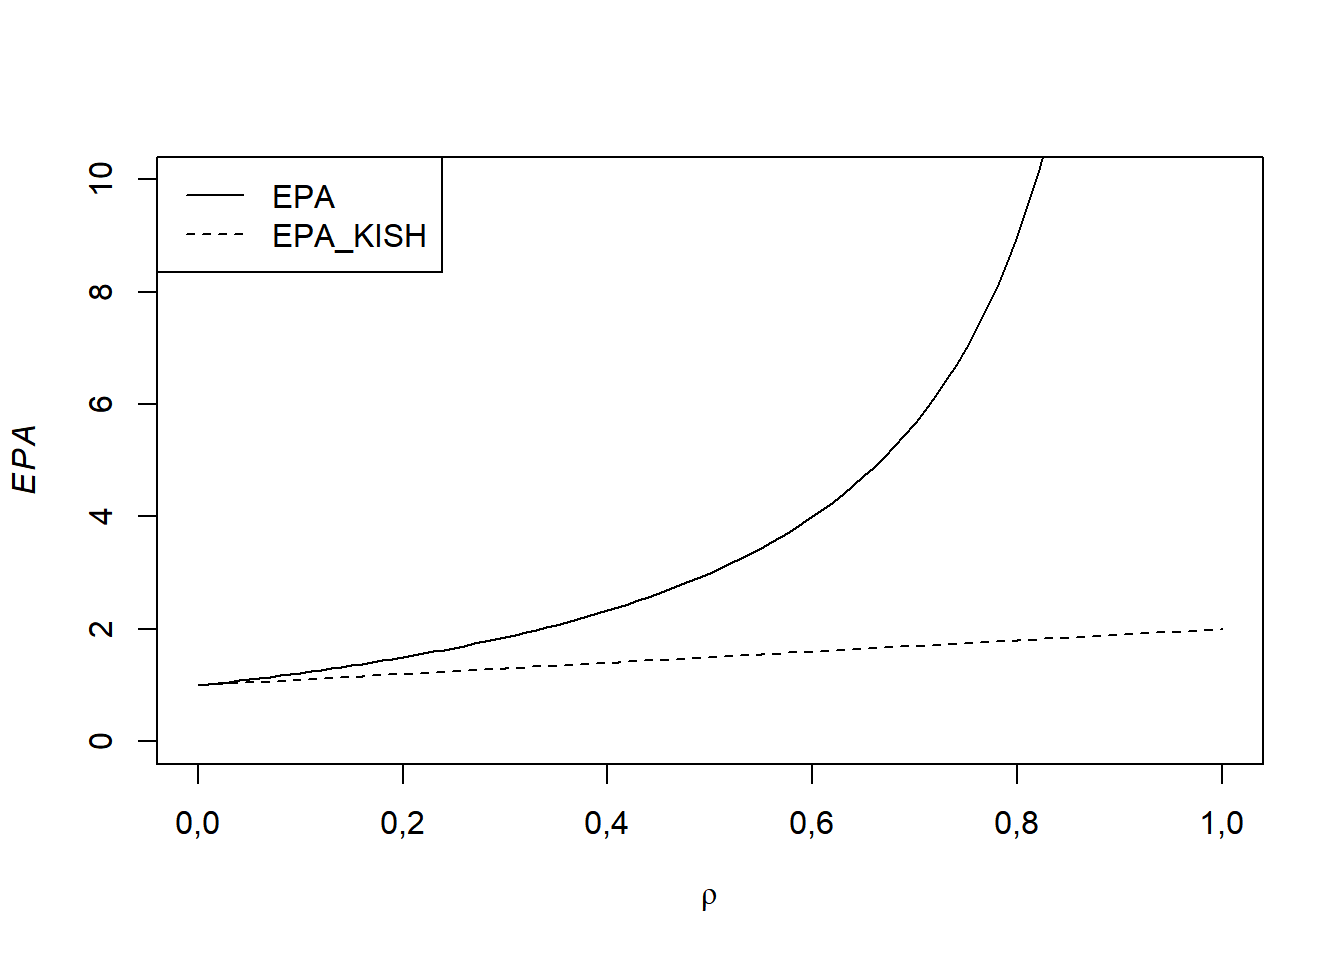
\includegraphics{04-Cap4_files/figure-latex/epacong-1.pdf}
\caption{\label{fig:epacong}Valores de EPA e EPA de Kish para conglomeração}
\end{figure}

Este exemplo ilustra bem dois aspectos distintos do uso de medidas como
o efeito de plano amostral. O primeiro é que as duas medidas são
distintas,
\texttt{embora\ os\ respectivos\ estimadores\ baseados\ numa\ particular\ amostra\ coincidam}.
No caso particular deste exemplo, o
\(\mathbf{EPA}_{Kish}\left( \hat{\theta}\right)\) cresce pouco com o
valor do coeficiente de correlação intraclasse \(\rho\), o que implica
que um plano amostral conglomerado como o adotado (seleção ao acaso de
um par da população) seria menos eficiente que um plano amostral
aleatório simples (seleção de duas unidades ao acaso da população), mas
a perda de eficiência seria modesta. Já se o interesse é medir, a
posteriori, o efeito da má especificação do plano amostral no estimador
de variância, o impacto, medido pelo
\(\mathbf{EPA}\left( \hat{\theta},v_{0}\right)\), seria muito maior.

Vale ainda notar que o \(\mathbf{EPA}\left( \hat{\theta},v_{0}\right)\)
mede o impacto da má especificação do plano amostral ou do modelo para a
estrutura populacional. Neste exemplo, ignorar a estrutura da população
(o fato de que as observações são pareadas) poderia provocar
subestimação da variância do estimador de média, que seria tanto maior
quanto maior fosse o coeficiente de correlação intraclasse \(\rho\).
Efeitos como esse são comuns também devido ao planejamento amostral,
mesmo em populações onde a conglomeração é imposta artificialmente pelo
amostrista.

\section{Intervalos de Confiança e Testes de Hipóteses}\label{icth}

A partir da estimativa pontual \(\hat{\theta}\) de um parâmetro
\(\theta\) (da população finita ou do modelo de superpopulação) é
possível construir um intervalo de confiança de nível de confiança
aproximado \(\left( 1-\alpha \right)\) a partir da distribuição
assintótica de \[
t_{0}=\frac{\hat{\theta}-\theta }{v_{0}^{1/2}} 
\] que, sob a hipótese de que as observações são IID, frequentemente é
\(N\left( 0;1\right)\).

Neste caso, um intervalo de confiança de nível de confiança aproximado
\(\left( 1-\alpha \right)\) é dado por
\(\left[ \hat{\theta}-z_{\alpha /2}v_{0}^{1/2},\hat{\theta}+z_{\alpha /2}v_{0}^{1/2}\right]\),
onde \(z_{\alpha }\) é definido por
\(\int_{z_{\alpha }}^{+\infty }\varphi\left( t\right) dt=\alpha\) , onde
\(\varphi\) é a função de densidade da distribuição normal padrão.

Vamos analisar o efeito de um plano amostral complexo sobre o intervalo
de confiança. No caso de um plano amostral complexo, a distribuição que
é aproximadamente normal é a de \[
\frac{\hat{\theta}-\theta }{\left[ \widehat{V}_{VERD}\left( \hat{\theta}\right) \right] ^{1/2}}. 
\]

Por outro lado, para obter a variância da distribuição assintótica de
\(t_{0}\) note que \[
\frac{\hat{\theta}-\theta }{v_{0}^{1/2}}=\frac{\hat{\theta}-\theta }{\left[ 
\widehat{V}_{VERD}\left( \hat{\theta}\right) \right] ^{1/2}}\times \frac{
\left[ \widehat{V}_{VERD}\left( \hat{\theta}\right) \right] ^{1/2}}{
v_{0}^{1/2}}\;. 
\]

Como o primeiro fator tende para uma \(N\left( 0;1\right)\), a variância
assintótica de \(t_{0}\) é aproximadamente igual ao quadrado do segundo
fator, isto é, a
\(\frac{\widehat{V}_{VERD}\left( \hat{\theta}\right) }{v_{0}}\) que é um
estimador para \(\mathbf{EPA}\left( \hat{\theta},v_{0}\right)\). Porém
quando a amostra é grande esse valor aproxima o
\(\mathbf{EPA}\left( \hat{\theta},v_{0}\right) =\frac{V_{VERD}\left( \hat{\theta}\right) }{E_{VERD}\left( v_{0}\right) }\),
pois \(v_{0}\) é aproximadamente igual a \(E_{VERD}\left( v_{0}\right)\)
e \(\widehat{V}_{VERD}\left( \hat{\theta}\right)\) é aproximadamente
igual a \(V_{VERD}\left( \hat{\theta}\right)\). Logo temos que a
distribuição assintótica verdadeira de \(t_{0}\) é dada por \[
t_{0}\sim N\left[ 0;\mathbf{EPA}\left( \hat{\theta},v_{0}\right)
\right] \;. 
\]

Dependendo do valor de \(\mathbf{EPA}\left( \hat{\theta},v_{0}\right)\),
o intervalo de confiança baseado na distribuição assintótica verdadeira
de \(t_{0}\) pode ser bem distinto daquele baseado na distribuição
assintótica obtida sob a hipótese de observações IID. Em geral, a
probabilidade de cobertura assintótica do intervalo
\(\left[\hat{\theta}-z_{\alpha /2}v_{0}^{1/2}, \hat{\theta}+z_{\alpha/2}v_{0}^{1/2}\right]\)
será aproximadamente igual a

\[
2\Phi \left( z_{\alpha /2}/\left[ \mathbf{EPA}\left( \hat{\theta}
,v_{0}\right) \right] ^{1/2}\right) -1\;\;, 
\] onde \(\Phi\) é a função de distribuição acumulada de uma
\(N\left( 0;1\right)\). Calculamos esta probabilidade para alguns
valores do \(\mathbf{EPA}\), que apresentamos na Tabela
\ref{tab:procob}.

\begin{longtable}[]{@{}lll@{}}
\caption{\label{tab:procob} Probabilidades de cobertura para níveis nominais
de 95\% e 99\%}\tabularnewline
\toprule
\(\mathbf{EPA}\left( \hat{\theta},v_{0}\right)\) & \(1-\alpha=0.95\) &
\(1-\alpha=0.99\)\tabularnewline
\midrule
\endfirsthead
\toprule
\(\mathbf{EPA}\left( \hat{\theta},v_{0}\right)\) & \(1-\alpha=0.95\) &
\(1-\alpha=0.99\)\tabularnewline
\midrule
\endhead
0,90 & 0,96 & 0,99\tabularnewline
0,95 & 0,96 & 0,99\tabularnewline
1,0 & 0,95 & 0,99\tabularnewline
1,5 & 0,89 & 0,96\tabularnewline
2,0 & 0,83 & 0,93\tabularnewline
2,5 & 0,78 & 0,90\tabularnewline
3,0 & 0,74 & 0,86\tabularnewline
3,5 & 0,71 & 0,83\tabularnewline
4,0 & 0,67 & 0,80\tabularnewline
\bottomrule
\end{longtable}

À medida que o valor do \(\mathbf{EPA}\left( \hat{\theta},v_{0}\right)\)
aumenta, a probabilidade real de cobertura diminui, sendo menor que o
valor nominal para valores de
\(\mathbf{EPA}\left( \hat{\theta},v_{0}\right)\) maiores que 1.

Utilizando a correspondência existente entre intervalos de confiança e
testes de hipóteses, podemos derivar os níveis de significância nominais
e reais subtraindo de \(1\) os valores da Tabela \ref{tab:procob}. Por
exemplo, para \(\alpha =0,05\) e
\(\mathbf{EPA}\left( \hat{\theta},v_{0}\right) =2\), o nível de
significância real seria aproximadamente \(1-0,83=0,17\).

\BeginKnitrBlock{example}
\protect\hypertarget{exm:exebin}{}{\label{exm:exebin} }Teste de hipótese
sobre proporção
\EndKnitrBlock{example} Vamos considerar um exemplo hipotético de teste
de hipótese sobre uma proporção, semelhante ao de \citep{Sud76},
apresentado em p.~196, \citep{lethonen}. Uma amostra de \(m=50\)
conglomerados é extraída de uma grande população de empresas industriais
(conglomerados). Suponhamos que cada empresa \(i=1,\ldots ,50\) da
amostra tenha \(n_{i}=20\) empregados. O tamanho total da amostra de
empregados (unidades elementares) é \(n=\sum_{i}n_{i}=1.000\). Queremos
estudar o acesso dos trabalhadores das empresas a planos de saúde.

Usando-se conhecimento do ano anterior, foi estabelecida a hipótese de
que a proporção de trabalhadores cobertos por planos de saúde é
\(80\%\), ou seja \(H_{0}:p=p_{0}=0,8\). Vamos adotar o nível de
significância \(\alpha =5\%\).

A estimativa obtida na pesquisa foi \(\widehat{p}=n_{A}/n=0,84\), onde
\(n_{A}=840\) é o número de trabalhadores na amostra com acesso a planos
de saúde. Ignorando o plano amostral e a conglomeração das unidades
elementares na população, podemos considerar um teste binomial e usar a
aproximação normal \(N(0;1)\) para a estatística de teste

\begin{equation}
Z=|\widehat{p}-p_{0}|/\sqrt{p_{0}\left( 1-p_{0}\right) /n},  \label{eq:epa4}
\end{equation}

onde o denominador é o desvio padrão da estimativa \(\widehat{p}\) sob a
hipótese nula.

Vamos calcular o valor da estatística \(Z\), supondo que tenha sido
usada amostragem aleatória simples com reposição (AASC) de empregados.
Vamos também considerar uma abordagem baseada no plano amostral de
conglomerados. O desvio padrão de \(\widehat{p}\), no denominador de
\(Z\), será baseado na hipótese de distribuição binomial, com tamanhos
amostrais diferentes para as duas abordagens.

Para o teste baseado na amostragem aleatória simples, ignoramos a
conglomeração e usamos na fórmula do desvio padrão o tamanho total da
amostra de unidades elementares (empregados), isto é, \(n=1.000\). O
valor da estatística de teste \(Z\) definida em \eqref{eq:epa4} é,
portanto,

\begin{equation}
Z_{bin}=|0,84-0,8|/\sqrt{0,8\left( 1-0,8\right) /1.000}=3,162>Z_{0,025}=1,96
\label{eq:epa5}
\end{equation}

onde \(\sqrt{0,8\left( 1-0,8\right) /1.000}=0,0126\) é o desvio padrão
de \(\widehat{p}\) sob a hipótese nula. Este~resultado sugere a rejeição
da hipótese \(H_{0}\).

Por outro lado, é razoável admitir que se uma empresa for coberta por
plano de saúde, cada empregado dessa empresa terá acesso ao plano. Essa
é uma informação importante que foi ignorada no teste anterior. De fato,
selecionar mais de uma pessoa numa empresa não aumenta nosso
conhecimento sobre a cobertura por plano de saúde no local. Portanto, o
\texttt{tamanho\ efetivo} da amostra é \(\overline{n}=50\) , em
contraste com o valor \(1.000\) usado no teste anterior. O termo
\texttt{tamanho\ efetivo} foi introduzido em \citep{Kish65} para
designar o tamanho de uma amostra aleatória simples necessário para
estimar \(p\) com a mesma precisão obtida por uma amostra conglomerada
de tamanho \(n\) (neste caso, igual a \(1.000\)) unidades elementares.

Usando o tamanho efetivo de amostra, temos a estatística de teste
baseada no plano amostral verdadeiro \[
Z_{p}=|\widehat{p}-p_{0}|/\sqrt{p_{0}\left( 1-p_{0}\right) /50}=0,707 ,
\] onde o valor \(\sqrt{0,8\left( 1-0,8\right) /50}=0,0566\) é muito
maior que o valor do desvio padrão obtido no teste anterior. Portanto, o
valor observado de \(Z_{p}\) é menor que o de \(Z_{bin}\), e o novo
teste sugere a não rejeição da mesma hipótese nula.

Neste exemplo, portanto, se verifica que ignorar a conglomeração pode
induzir a uma decisão incorreta de rejeitar a hipótese nula, quando a
mesma não seria rejeitada se o plano amostral fosse corretamente
incorporado na análise. Efeitos desse tipo são mais difíceis de
antecipar para inferência analítica, particularmente quando os planos
amostrais empregados envolvem combinação de estratificação,
conglomeração e probabilidades desiguais de seleção. Por essa razão, a
recomendação é procurar sempre considerar o plano amostral na análise,
ao menos como forma de verificar se as conclusões obtidas por formas
ingênuas de análise ignorando os pesos e plano amostral são as mesmas.

\section{Efeitos Multivariados de Plano
Amostral}\label{efeitos-multivariados-de-plano-amostral}

O conceito de efeito de plano amostral introduzido em \eqref{eq:epa2} é
relativo a inferências sobre um parâmetro univariado \(\theta\).
Consideremos agora o problema de estimação de um vetor
\(\mathbf{\theta}\) de \(K\) parâmetros. Seja \(\mathbf{\hat{\theta}}\)
um estimador de \(\mathbf{\theta}\) e seja \(\mathbf{V}_{0}\) um
estimador da matriz \(K\times K\) de covariância de
\(\mathbf{\hat{\theta}}\), baseado nas hipóteses de independência e
igualdade de distribuição das observações (IID), ou equivalentemente, de
amostragem aleatória simples com reposição (AASC). é possível
generalizar a equação \eqref{eq:epa2}, definindo o
\texttt{efeito\ multivariado\ do\ plano\ amostral\ de}
\(\mathbf{\hat{\theta}}\) \textbf{e} \(\mathbf{V}_{0}\) como

\begin{equation}
\mathbf{EMPA}(\mathbf{\hat{\theta},V}_{0})=\mathbf{\Delta =E}_{VERD}\left( 
\mathbf{V}_{0}\right) ^{-1}\mathbf{V}_{VERD}(\mathbf{\hat{\theta}),}
\label{eq:epa6}
\end{equation}

onde \(\mathbf{E}_{VERD}\left( \mathbf{V}_{0}\right)\) é o valor
esperado de \(\mathbf{V}_{0}\) e,
\(\mathbf{V}_{VERD}(\mathbf{\hat{\theta})}\) é a matriz de covariância
de \(\mathbf{\hat{\theta}}\), ambas calculadas com respeito `\{a\}
distribuição de aleatorização induzida pelo plano amostral efetivamente
utilizado, ou alternativamente sob o \texttt{modelo\ correto}.

Os autovalores \(\delta _{1}\geq \ldots \geq \delta _{K}\) da matriz
\(\mathbf{\Delta }\) são denominados
\texttt{efeitos\ generalizados\ do\ plano\ amostral}. A partir deles, e
utilizando resultados padrões de teoria das matrizes (p.64,
\citep{Johnson}) é possível definir limitantes para os efeitos
(univariados) do plano amostral para combinações lineares
\(\mathbf{c}^{^{\prime }}\widehat{\mathbf{\theta }}\) das componentes de
\(\widehat{\mathbf{\theta }}\). Temos os seguintes resultados:

\begin{eqnarray*}
\delta _{1} &=&\max \mathbf{EPA}(\mathbf{c}^{^{\prime }}\widehat{\mathbf{
\theta }}\mathbf{,c}^{^{\prime }}\mathbf{V}_{0}\mathbf{c)}, \\
\delta _{K} &=&\min \mathbf{EPA}(\mathbf{c}^{^{\prime }}\widehat{\mathbf{\theta }}\mathbf{,c}^{^{\prime }}\mathbf{V}_{0}\mathbf{c)}.
\end{eqnarray*}

No caso particular onde \(\mathbf{\Delta =I}_{K\times K}\) , temos
\(\delta_{1}=\ldots =\delta _{K}=1\) e os efeitos (univariados) do plano
amostral das combinações lineares para componentes de
\(\mathbf{\hat{\theta}}\) são todos iguais a \(1\). Para ilustrar esse
conceito, vamos reconsiderar o Exemplo \ref{exm:deffuni} de estimação de
médias com amostragem estratificada desproporcional anteriormente
apresentado, mas agora considerando a natureza multivariada do problema
(há duas variáveis de pesquisa).

\BeginKnitrBlock{example}
\protect\hypertarget{exm:deffmult}{}{\label{exm:deffmult} }Efeitos
Multivariados do Plano Amostral para as médias de Salários e de Receitas
\EndKnitrBlock{example}

Vamos considerar as variáveis Salário (em R\$ \(1.000\)) e Receita (em
R\$ \(1.000.000\)) definidas na população de empresas do Exemplo
\ref{exm:deffuni} e calcular a matriz
\(\mathbf{EMPA}\left( \mathbf{\hat{\theta},V}_{0}\right)\), onde
\(\mathbf{\hat{\theta}=}\left( \overline{SAL}_{w},\overline{REC}_{w}\right) ^{\prime }\).
Neste exemplo, os dados populacionais são conhecidos, e portanto podemos
calcular a covariância dos estimadores
\(\left( \overline{SAL}_{w},\overline{REC}_{w}\right)\). Usando a mesma
notação do Exemplo \ref{exm:deffuni}, temos que \[
COV_{AES}(\overline{SAL}_{w},\overline{REC}_{w}\mathbf{)=}\sum\limits_{h=1}^{2}W_{h}^{2}\frac{\left( 1-f_{h}\right) }{n_{h}}S_{SAL,REC}^{\left( h\right) } 
\] onde \[
S_{SAL,REC}^{\left( h\right) }=\frac{1}{N_{h}-1}\sum\limits_{i\in
U_{h}}\left( SAL_{hi}-\overline{SAL}_{h}\right) \left( REC_{hi}-\overline{REC
}_{h}\right) \;. 
\]

Substituindo os valores conhecidos na população das variáveis
\(SAL_{hi}\) e \(REC_{hi}\), obtemos para esta covariância o valor \[
COV_{AES}(\overline{SAL}_{w},\overline{REC}_{w}\mathbf{)=\;}3.2358
\] e portanto a matriz de variância
\(\mathbf{V}_{AES}(\overline{SAL}_{w},\overline{REC}_{w})\) dos
estimadores ponderados da média fica igual a

\begin{verbatim}
       SAL   REC
SAL 244,18 3,236
REC   3,24 0,435
\end{verbatim}

onde os valores das variâncias em \eqref{eq:epa7} foram os calculados no
Exemplo \ref{exm:deffuni} e coincidem, respectivamente, com os valores
usados nos numeradores de
\(\mathbf{EPA}\left( \overline{SAL}_{w}\right)\) e de
\(\mathbf{EPA}\left( \overline{REC}_{w}\right)\) lá apresentados. Para
calcular o \(\mathbf{EMPA}(\mathbf{\hat{\theta},V}_{0})\) é preciso
agora obter \(\mathbf{E}_{VERD}\left(\mathbf{V}_{0}\right)\).

Neste exemplo, a matriz de efeito do plano amostral
\(\mathbf{EMPA}(\mathbf{\hat{\theta},V}_{0})=\mathbf{\Delta }\) pode
também ser calculada através de simulação, de modo análogo ao que foi
feito no Exemplo \ref{exm:deffuni}. Para isto, foram utilizadas outras
\(500\) amostras de tamanho \(60\) segundo o plano amostral descrito no
Exemplo \ref{exm:deffuni}. Para cada uma das \(500\) amostras foram
calculadas estimativas:

\begin{enumerate}
\def\labelenumi{\arabic{enumi}.}
\item
  da variância da média amostral ponderada do salário e da receita
  assumindo observações IID;
\item
  da covariância entre médias ponderadas do salário e da receita
  assumindo observações IID;
\item
  da variância da média amostral ponderada do salário e da receita
  considerando o plano amostral verdadeiro;
\item
  da covariância entre médias ponderadas do salário e da receita
  considerando o plano amostral verdadeiro.
\end{enumerate}

A partir da simulação foram obtidos os seguintes resultados:

\begin{itemize}
\tightlist
\item
  A matriz de covariância das médias amostrais ponderadas de salário e
  da receita, assumindo observações IID \(E_{AES}\left(V_{0}\right)\):
\end{itemize}

\begin{verbatim}
       SAL   REC
SAL 1720,0 26,78
REC   26,8  1,21
\end{verbatim}

\begin{itemize}
\tightlist
\item
  A matriz de covariância das médias ponderadas de salário e da receita
  considerando o plano amostral verdadeiro
  \(V_{AES}\left(\hat{\theta}\right)\):
\end{itemize}

\begin{verbatim}
       SAL   REC
SAL 245,19 3,172
REC   3,17 0,401
\end{verbatim}

\begin{itemize}
\tightlist
\item
  A matriz \(\Delta\) definida em \eqref{eq:epa6}
\end{itemize}

\(\Delta = \left[ E_{AES}\left( V_{0}\right)\right]^{-1}V_{AES}(\hat{\theta})\)

\begin{verbatim}
        sal      rec
[1,]  0,155 -0,00509
[2,] -0,817  0,44506
\end{verbatim}

Os autovalores 1 e 1,02 de \(\mathbf{\Delta}\) fornecem os efeitos
generalizados do plano amostral.

Da mesma forma que o \(\mathbf{EPA}\left( \hat{\theta},v_{0}\right)\)
definido em \eqref{eq:epa2} para o caso uniparamétrico foi utilizado para
corrigir níveis de confiança de intervalos e níveis de significância de
testes, o \(\mathbf{EMPA}(\mathbf{\hat{\theta},V}_{0})\) definido em
\eqref{eq:epa6} pode ser utilizado para corrigir níveis de confiança de
regiões de confiança e níveis de significância de testes de hipóteses no
caso multiparamétrico. Para ilustrar, vamos considerar o problema de
testar a hipótese \(H_{0}:\mathbf{\mu }=\mathbf{\mu }_{0}\), onde
\(\mathbf{\mu }\) é o vetor de médias de um vetor de variáveis de
pesquisa \(\mathbf{y}\). A estatística de teste usualmente adotada para
este caso é a \(T^{2}\) de Hottelling dada por

\begin{equation}
T^{2}=n\left( \mathbf{\bar{y}-\mu }_{0}\right) ^{^{\prime }}\mathbf{S}
_{y}^{-1}\left( \mathbf{\bar{y}-\mu }_{0}\right) , \label{eq:epa11} 
\end{equation}

onde

\begin{eqnarray*}
\mathbf{\bar{y}} &=&\frac{1}{n}\sum\limits_{i\in s}\mathbf{y}_{i},\quad 
\mathbf{S}_{y}=\frac{1}{n-1}\sum\limits_{i\in s}\left( \mathbf{y}_{i}-
\mathbf{\bar{y}}\right) \left( \mathbf{y}_{i}-\mathbf{\bar{y}}\right)
^{^{\prime }},\mbox{ e } \\
\mathbf{\mu }_{0} &=&\left( \mu _{10},\mu _{20},\ldots ,\mu _{K0}\right)
^{^{\prime }}\;\;.
\end{eqnarray*}

Se as observações \(\mathbf{y}_{i}\) são IID normais, a estatística
\(T^{2}\) tem a distribuição
\(\frac{\left( n-1\right) }{\left( n-K\right)}\mathbf{F}\left( K;n-K\right)\)
sob \(H_{0}\), onde \(\mathbf{F}\left( K;n-K\right)\) denota uma
variável aleatória com distribuição \(\mathbf{F}\) com \(K\) e
\(\left( n-K\right)\) graus de liberdade. Mesmo se as observações
\(\mathbf{y}_{i}\) não forem normais, \(T^{2}\) tem distribuição
assintótica \(\chi ^{2}\left(K\right)\) quando \(n\rightarrow \infty\),
\citep{Johnson}, p.191.

Contudo, se for utilizado um plano amostral complexo, \(T^{2}\) tem
aproximadamente a distribuição da variável \(\sum\limits_{i=1}^{K}\)
\(\delta _{i}Z_{i}^{2}\), onde \(Z_{1},\ldots ,Z_{K}\) são variáveis
aleatórias independentes com distribuição normal padrão e os
\(\delta _{i}\) são os autovalores da matriz
\(\mathbf{\Delta }=\Sigma _{AAS}^{-1}\Sigma\), onde
\(\Sigma _{AAS}=E_{p}(\mathbf{S}_{y}/n)\) e
\(\Sigma =V_{p}(\mathbf{\bar{y})}\).

Vamos analisar o efeito do plano amostral sobre o nível de significância
deste teste. Para simplificar, consideremos o caso em que
\(\delta _{1}=\ldots =\delta _{K}=\delta\). Neste caso, o nível de
significância real é dado aproximadamente por

\begin{equation}
P\left(\chi ^{2}\left( K\right) >\chi _{\alpha }^{2}\left( K\right) /\delta\right)  \label{eq:epa12}
\end{equation}

onde \(\chi _{\alpha }^{2}\left( K\right)\) é o quantil superior
\(\alpha\) de uma distribuição \(\chi ^{2}\) com \(K\) graus de
liberdade, isto é, o valor tal que
\(P\left[ \chi ^{2}\left( K\right) >\chi _{\alpha}^{2}\left( K\right) \right] =\alpha\)
.

A Tabela \ref{tab:nivsig} apresenta os níveis de significância reais
para \(\alpha =5\%\) para vários valores de \(K\) e \(\delta\). Mesmo
quando os valores dos \(\delta _{i}\) são distintos, os valores da
Tabela \ref{tab:nivsig} podem ser devidamente interpretados. Para isso,
consideremos o \(p\)valor do teste da hipótese
\(H_{0}:\mathbf{\mu }=\mathbf{\mu }_{0}\), sob a hipótese de amostragem
aleatória simples com reposição e sob o plano amostral efetivamente
utilizado. Por definição este valor é dado por \[
p\mbox{valor}_{AAS}\left( \mathbf{\bar{y}}\right) =P\left[ \chi ^{2}\left(
K\right) >\left( \mathbf{\bar{y}-\mu }_{0}\right) ^{^{\prime }}\mathbf{
\Sigma }_{AAS}^{-1}\left( \mathbf{\bar{y}-\mu }_{0}\right) \right] 
\] e \(H_{0}\) é rejeitada com nível de significância \(\alpha\) se
valor-\(p\) \(_{AAS}<\alpha\).

O verdadeiro valor-\(p\) pode ser definido analogamente como

\begin{equation}
p\mbox{valor}_{VERD}\left( \mathbf{\bar{y}}\right) =P\left[ \chi ^{2}\left(K\right) >\left( \mathbf{\bar{y}-\mu }_{0}\right) ^{^{\prime }}\mathbf{\Sigma }_{VERD}^{-1}\left( \mathbf{\bar{y}-\mu }_{0}\right) \right] \;.
\label{eq:epa13}
\end{equation}

Os valores na Tabela \ref{tab:nivsig} podem ser usados para quantificar
a diferença entre estes valores-\(p\). Consideremos a região crítica do
teste de nível \(\alpha\) baseado na hipótese de AAS:

\begin{eqnarray}
RC_{AAS}\left( \mathbf{\bar{y}}\right) &=&\left\{ \mathbf{\bar{y}:}\left( 
\mathbf{\bar{y}-\mu }_{0}\right) ^{^{\prime }}\mathbf{\Sigma }
_{AAS}^{-1}\left( \mathbf{\bar{y}-\mu }_{0}\right) >\chi _{\alpha
}^{2}\left( K\right) \right\} \label{eq:epa14}  \\
&=&\left\{ \mathbf{\bar{y}:}p\mbox{valor}_{AAS}\left( \mathbf{\bar{y}}
\right) <\alpha \right\}.  \nonumber
\end{eqnarray}

Pode-se mostrar que o máximo de
\(p\)valor\(_{VERD}\left( \mathbf{\bar{y}}\right)\) quando
\(\mathbf{\bar{y}}\) pertence à
\(RC_{AAS}\left( \mathbf{\bar{y}}\right)\) é dado por:

\begin{equation}
\max_{\mathbf{\bar{y}\in }RC_{AAS}\left( \mathbf{\bar{y}}\right) }p
\mbox{valor}_{VERD}\left( \mathbf{\bar{y}}\right) =P\left( \chi ^{2}\left(K\right) >\chi _{\alpha }^{2}\left( K\right) /\delta _{1}\right).
\label{eq:epa15}
\end{equation}

Observe que o segundo membro de \eqref{eq:epa15} é da mesma forma que o
segundo membro de \eqref{eq:epa12}. Logo, os valores da Tabela
\ref{tab:nivsig} podem ser interpretados como valores máximos de
\(p\)valor\(_{VERD}\left( \mathbf{\bar{y}}\right)\) para
\(\mathbf{\bar{y}}\) na região
\(RC_{AAS}\left(\mathbf{\bar{y}}\right)\), considerando-se
\(\delta_{1}\) no lugar de \(\delta\).

\begin{longtable}[]{@{}cllrr@{}}
\caption{\label{tab:nivsig} Níveis de significância (\%) verdadeiros do
teste T2 para o nível nominal de 5\% assumindo autovalores iguais a
\(\delta\).}\tabularnewline
\toprule
& & K & &\tabularnewline
\midrule
\endfirsthead
\toprule
& & K & &\tabularnewline
\midrule
\endhead
\(\delta\) & 1 & 2 & 3 & 4\tabularnewline
0,9 & 4 & 4 & 3 & 3\tabularnewline
1,0 & 5 & 5 & 5 & 5\tabularnewline
1,5 & 11 & 14 & 16 & 19\tabularnewline
2,0 & 17 & 22 & 27 & 32\tabularnewline
2,5 & 22 & 30 & 37 & 44\tabularnewline
3,0 & 26 & 37 & 46 & 53\tabularnewline
\bottomrule
\end{longtable}

\section{Laboratório de R}\label{laboratorio-de-r-1}

Utilizando o R, obtemos a seguir alguns resultados descritos nos
Exemplos \ref{exm:deffuni} e \ref{exm:deffmult}. Na simulação, usamos a
library \texttt{sampling} \citep{R-sampling} para gerar amostras
estratificadas de tamanho 30, com estratos definidos na Tabela
\ref{tab:estempr}, para obter os valores nas Tabelas \ref{tab:proestmed}
e \ref{tab:varest}.

\begin{Shaded}
\begin{Highlighting}[]
\CommentTok{# carrega library}
\KeywordTok{library}\NormalTok{(survey)}
\CommentTok{# carrega dados}
\KeywordTok{library}\NormalTok{(anamco)}
\NormalTok{popul_dat <-}\StringTok{ }\NormalTok{popul}
\NormalTok{N <-}\StringTok{ }\KeywordTok{nrow}\NormalTok{(popul_dat)}
\NormalTok{n1 <-}\StringTok{ }\DecValTok{30}
\NormalTok{n2 <-}\StringTok{ }\DecValTok{30}
\NormalTok{nh =}\StringTok{ }\KeywordTok{c}\NormalTok{(n1, n2)}
\NormalTok{n <-}\StringTok{ }\KeywordTok{sum}\NormalTok{(nh)}
\NormalTok{Nh <-}\StringTok{ }\KeywordTok{table}\NormalTok{(popul_dat}\OperatorTok{$}\NormalTok{estrat)}
\NormalTok{fh <-}\StringTok{ }\NormalTok{nh}\OperatorTok{/}\NormalTok{Nh}
\NormalTok{Wh <-}\StringTok{ }\NormalTok{Nh}\OperatorTok{/}\NormalTok{N}
\NormalTok{f <-}\StringTok{ }\NormalTok{n}\OperatorTok{/}\NormalTok{N}
\NormalTok{popul_dat}\OperatorTok{$}\NormalTok{sal <-}\StringTok{ }\NormalTok{popul_dat}\OperatorTok{$}\NormalTok{sal}\OperatorTok{/}\DecValTok{1000}
\NormalTok{popul_dat}\OperatorTok{$}\NormalTok{rec <-}\StringTok{ }\NormalTok{popul_dat}\OperatorTok{$}\NormalTok{rec}\OperatorTok{/}\FloatTok{1e+06}
\KeywordTok{library}\NormalTok{(sampling)}
\CommentTok{# define espaços para salvar resultados}
\NormalTok{est_aas <-}\StringTok{ }\KeywordTok{c}\NormalTok{(}\DecValTok{0}\NormalTok{, }\DecValTok{0}\NormalTok{)}
\NormalTok{est_aes <-}\StringTok{ }\KeywordTok{c}\NormalTok{(}\DecValTok{0}\NormalTok{, }\DecValTok{0}\NormalTok{)}
\NormalTok{cov_mat_aas_est <-}\StringTok{ }\KeywordTok{matrix}\NormalTok{(}\DecValTok{0}\NormalTok{, }\DecValTok{2}\NormalTok{, }\DecValTok{2}\NormalTok{)}
\NormalTok{cov_mat_aes_est <-}\StringTok{ }\KeywordTok{matrix}\NormalTok{(}\DecValTok{0}\NormalTok{, }\DecValTok{2}\NormalTok{, }\DecValTok{2}\NormalTok{)}
\KeywordTok{set.seed}\NormalTok{(}\DecValTok{123}\NormalTok{)}
\CommentTok{# gera amostras com dois estratos de tamanho 30}
\ControlFlowTok{for}\NormalTok{ (i }\ControlFlowTok{in} \DecValTok{1}\OperatorTok{:}\DecValTok{500}\NormalTok{) \{}
\NormalTok{  s <-}\StringTok{ }\KeywordTok{strata}\NormalTok{(popul_dat, }\StringTok{"estrat"}\NormalTok{, }\KeywordTok{c}\NormalTok{(}\DecValTok{30}\NormalTok{, }\DecValTok{30}\NormalTok{), }\DataTypeTok{method =} \StringTok{"srswor"}\NormalTok{)}
\NormalTok{  dados <-}\StringTok{ }\KeywordTok{getdata}\NormalTok{(popul_dat, s)}
  \CommentTok{# média amostral de salário e de receita}
\NormalTok{  est_aas <-}\StringTok{ }\NormalTok{est_aas }\OperatorTok{+}\StringTok{ }\KeywordTok{c}\NormalTok{(}\KeywordTok{mean}\NormalTok{(dados}\OperatorTok{$}\NormalTok{sal), }\KeywordTok{mean}\NormalTok{(dados}\OperatorTok{$}\NormalTok{rec))}
  \CommentTok{# estimador v0}
\NormalTok{  cov_mat_aas_est <-}\StringTok{ }\NormalTok{cov_mat_aas_est }\OperatorTok{+}\StringTok{ }\NormalTok{(}\DecValTok{1} \OperatorTok{-}\StringTok{ }\NormalTok{f) }\OperatorTok{*}\StringTok{ }\KeywordTok{cov}\NormalTok{(}\KeywordTok{cbind}\NormalTok{(dados}\OperatorTok{$}\NormalTok{sal, }
\NormalTok{    dados}\OperatorTok{$}\NormalTok{rec))}\OperatorTok{/}\NormalTok{n}
  
  \CommentTok{# vhat_aes estimador não-viciado}
\NormalTok{  popul_plan <-}\StringTok{ }\KeywordTok{svydesign}\NormalTok{(}\OperatorTok{~}\DecValTok{1}\NormalTok{, }\DataTypeTok{strata =} \OperatorTok{~}\NormalTok{estrat, }\DataTypeTok{data =}\NormalTok{ dados, }
    \DataTypeTok{fpc =} \OperatorTok{~}\NormalTok{Prob)}
  \CommentTok{# estimador não-viciado da média de salario e receita}
\NormalTok{  sal_rec_aes_est <-}\StringTok{ }\KeywordTok{svymean}\NormalTok{(}\OperatorTok{~}\NormalTok{sal }\OperatorTok{+}\StringTok{ }\NormalTok{rec, popul_plan)}
\NormalTok{  est_aes <-}\StringTok{ }\NormalTok{est_aes }\OperatorTok{+}\StringTok{ }\KeywordTok{coef}\NormalTok{(sal_rec_aes_est)}
\NormalTok{  cov_mat_aes_est <-}\StringTok{ }\NormalTok{cov_mat_aes_est }\OperatorTok{+}\StringTok{ }\KeywordTok{attr}\NormalTok{(sal_rec_aes_est, }
    \StringTok{"var"}\NormalTok{)}
\NormalTok{\}}

\CommentTok{# média populacional}

\NormalTok{med_pop <-}\StringTok{ }\KeywordTok{round}\NormalTok{(}\KeywordTok{c}\NormalTok{(}\KeywordTok{mean}\NormalTok{(popul_dat}\OperatorTok{$}\NormalTok{sal), }\KeywordTok{mean}\NormalTok{(popul_dat}\OperatorTok{$}\NormalTok{rec)),}\DecValTok{3}\NormalTok{)}


\CommentTok{# Calcula médias das estimativas na simulação}

\NormalTok{## Média das estimativas pontuais para as 500 amostras aas}
\NormalTok{mean_est_aas <-}\StringTok{ }\KeywordTok{round}\NormalTok{(est_aas}\OperatorTok{/}\DecValTok{500}\NormalTok{,}\DecValTok{3}\NormalTok{)}
\NormalTok{mean_est_aas}
\end{Highlighting}
\end{Shaded}

\begin{verbatim}
## [1] 163,50   4,17
\end{verbatim}

\begin{Shaded}
\begin{Highlighting}[]
\NormalTok{## Média das estimativas pontuais para as 500 amostras aes}
\NormalTok{mean_est_aes <-}\StringTok{ }\KeywordTok{round}\NormalTok{(est_aes}\OperatorTok{/}\DecValTok{500}\NormalTok{,}\DecValTok{3}\NormalTok{)}
\NormalTok{mean_est_aes}
\end{Highlighting}
\end{Shaded}

\begin{verbatim}
##   sal   rec 
## 78,07  2,06
\end{verbatim}

\begin{Shaded}
\begin{Highlighting}[]
\CommentTok{# Média das estimativas de matriz de covariância para as 500}
\CommentTok{# amostras aas}
\NormalTok{mean_cov_mat_aas_est <-}\StringTok{ }\KeywordTok{round}\NormalTok{(cov_mat_aas_est}\OperatorTok{/}\DecValTok{500}\NormalTok{, }\DecValTok{3}\NormalTok{)}
\NormalTok{mean_cov_mat_aas_est}
\end{Highlighting}
\end{Shaded}

\begin{verbatim}
##        [,1]  [,2]
## [1,] 1720,0 26,78
## [2,]   26,8  1,21
\end{verbatim}

\begin{Shaded}
\begin{Highlighting}[]
\CommentTok{# Média das estimativas de matriz de covariância para as 500}
\CommentTok{# amostras aes}
\NormalTok{mean_cov_mat_aes_est <-}\StringTok{ }\KeywordTok{round}\NormalTok{(cov_mat_aes_est}\OperatorTok{/}\DecValTok{500}\NormalTok{, }\DecValTok{3}\NormalTok{)}
\NormalTok{mean_cov_mat_aes_est}
\end{Highlighting}
\end{Shaded}

\begin{verbatim}
##        sal   rec
## sal 245,19 3,172
## rec   3,17 0,401
\end{verbatim}

\begin{Shaded}
\begin{Highlighting}[]
\NormalTok{## Matriz de covariância populacional}
\NormalTok{mat_cov_pop <-}\StringTok{ }\KeywordTok{by}\NormalTok{(popul_dat, popul_dat}\OperatorTok{$}\NormalTok{estrat, }\ControlFlowTok{function}\NormalTok{(t) }\KeywordTok{var}\NormalTok{(}\KeywordTok{cbind}\NormalTok{(t}\OperatorTok{$}\NormalTok{sal, }
\NormalTok{  t}\OperatorTok{$}\NormalTok{rec)))}
 


\NormalTok{## Matriz de covariância considerando o plano amostral}
\NormalTok{## verdadeiro}
\NormalTok{mat_cov_aleat_verd <-}\StringTok{ }\NormalTok{(Wh[}\DecValTok{1}\NormalTok{]}\OperatorTok{^}\DecValTok{2} \OperatorTok{*}\StringTok{ }\NormalTok{(}\DecValTok{1} \OperatorTok{-}\StringTok{ }\NormalTok{fh[}\DecValTok{1}\NormalTok{])}\OperatorTok{/}\NormalTok{nh[}\DecValTok{1}\NormalTok{]) }\OperatorTok{*}\StringTok{ }\NormalTok{mat_cov_pop[[}\DecValTok{1}\NormalTok{]] }\OperatorTok{+}\StringTok{ }
\StringTok{  }\NormalTok{(Wh[}\DecValTok{2}\NormalTok{]}\OperatorTok{^}\DecValTok{2} \OperatorTok{*}\StringTok{ }\NormalTok{(}\DecValTok{1} \OperatorTok{-}\StringTok{ }\NormalTok{fh[}\DecValTok{2}\NormalTok{])}\OperatorTok{/}\NormalTok{nh[}\DecValTok{2}\NormalTok{]) }\OperatorTok{*}\StringTok{ }\NormalTok{mat_cov_pop[[}\DecValTok{2}\NormalTok{]]}
\NormalTok{mat_cov_aleat_verd <-}\StringTok{ }\KeywordTok{round}\NormalTok{(mat_cov_aleat_verd,}\DecValTok{3}\NormalTok{)}


\NormalTok{## estimativa de efeitos generalizados do plano amostral}
\NormalTok{DELTA =}\StringTok{ }\KeywordTok{solve}\NormalTok{(mean_cov_mat_aas_est) }\OperatorTok\StringTok{ }\NormalTok{mean_cov_mat_aes_est}
\NormalTok{epa <-}\KeywordTok{round}\NormalTok{(}\KeywordTok{eigen}\NormalTok{(DELTA)}\OperatorTok{$}\NormalTok{values,}\DecValTok{3}\NormalTok{)}
\end{Highlighting}
\end{Shaded}

\BeginKnitrBlock{example}
\protect\hypertarget{exm:eqmean}{}{\label{exm:eqmean} }Teste da igualdade de
médias para duas populações
\EndKnitrBlock{example}

Para exemplificar o material descrito na Seção \ref{icth}, vamos
utilizar o data frame \texttt{amolim}, contendo dados da
\texttt{Amostra\ do\ Censo\ Experimental\ de\ Limeira}.

\begin{Shaded}
\begin{Highlighting}[]
\CommentTok{# carregar dados}
\KeywordTok{library}\NormalTok{(anamco)}
\KeywordTok{dim}\NormalTok{(amolim)}
\end{Highlighting}
\end{Shaded}

\begin{verbatim}
## [1] 706  14
\end{verbatim}

\begin{Shaded}
\begin{Highlighting}[]
\KeywordTok{names}\NormalTok{(amolim)}
\end{Highlighting}
\end{Shaded}

\begin{verbatim}
##  [1] "setor"  "np"     "domic"  "sexo"   "renda"  "lrenda" "raca"  
##  [8] "estudo" "idade"  "na"     "peso"   "domtot" "peso1"  "pesof"
\end{verbatim}

\begin{itemize}
\tightlist
\item
  Objeto de desenho para os dados da Amostra de Limeira:
\end{itemize}

\begin{Shaded}
\begin{Highlighting}[]
\KeywordTok{library}\NormalTok{(survey)}
\NormalTok{amolim.des<-}\KeywordTok{svydesign}\NormalTok{(}\DataTypeTok{id=}\OperatorTok{~}\NormalTok{setor}\OperatorTok{+}\NormalTok{domic, }\DataTypeTok{weights=}\OperatorTok{~}\NormalTok{pesof,}
  \DataTypeTok{data=}\NormalTok{amolim)}
\end{Highlighting}
\end{Shaded}

\begin{itemize}
\tightlist
\item
  Vamos estimar, a renda média por raça:
\end{itemize}

\begin{Shaded}
\begin{Highlighting}[]
\KeywordTok{svyby}\NormalTok{(}\OperatorTok{~}\NormalTok{renda, }\OperatorTok{~}\NormalTok{raca, amolim.des, svymean)}
\end{Highlighting}
\end{Shaded}

\begin{verbatim}
##   raca  renda    se
## 1    1 110406 11262
## 2    2  73560  8207
\end{verbatim}

\begin{itemize}
\tightlist
\item
  Vamos estimar, a renda média por sexo:
\end{itemize}

\begin{Shaded}
\begin{Highlighting}[]
\KeywordTok{svyby}\NormalTok{(}\OperatorTok{~}\NormalTok{renda, }\OperatorTok{~}\NormalTok{sexo, amolim.des, svymean)}
\end{Highlighting}
\end{Shaded}

\begin{verbatim}
##   sexo  renda    se
## 1    1 108746 11696
## 2    2  40039  4042
\end{verbatim}

\begin{itemize}
\tightlist
\item
  Vamos testar a igualdade de rendas por sexo:
\end{itemize}

\begin{Shaded}
\begin{Highlighting}[]
\KeywordTok{svyttest}\NormalTok{(renda }\OperatorTok{~}\StringTok{ }\NormalTok{sexo, amolim.des)}
\end{Highlighting}
\end{Shaded}

\begin{verbatim}
## 
##  Design-based t-test
## 
## data:  renda ~ sexo
## t = -6, df = 20, p-value = 5e-06
## alternative hypothesis: true difference in mean is not equal to 0
## sample estimates:
## difference in mean 
##             -68707
\end{verbatim}

\begin{itemize}
\tightlist
\item
  Vamos testar a igualdade de rendas por raça:
\end{itemize}

\begin{Shaded}
\begin{Highlighting}[]
\KeywordTok{svyttest}\NormalTok{(renda }\OperatorTok{~}\StringTok{ }\NormalTok{raca, amolim.des)}
\end{Highlighting}
\end{Shaded}

\begin{verbatim}
## 
##  Design-based t-test
## 
## data:  renda ~ raca
## t = -4, df = 20, p-value = 6e-04
## alternative hypothesis: true difference in mean is not equal to 0
## sample estimates:
## difference in mean 
##             -36846
\end{verbatim}

\chapter{Ajuste de Modelos Paramétricos}\label{ajmodpar}

\section{Introdução}\label{modpar1}

\section{Método de Máxima Verossimilhança
(MV)}\label{metodo-de-maxima-verossimilhanca-mv}

\section{Ponderação de Dados
Amostrais}\label{ponderacao-de-dados-amostrais}

\section{Método de Máxima Pseudo-Verossimilhança}\label{modpar3}

\section{Robustez do Procedimento
MPV}\label{robustez-do-procedimento-mpv}

\section{Desvantagens da Inferência de
Aleatorização}\label{desvantagens-da-inferencia-de-aleatorizacao}

\section{Laboratório de R}\label{laboratorio-de-r-2}

\chapter{Modelos de Regressão}\label{modreg}

\section{Modelo de Regressão Linear Normal}\label{modlinear}

\subsection{Especificação do Modelo}\label{especificacao-do-modelo}

\subsection{Pseudo-parâmetros do
Modelo}\label{pseudo-parametros-do-modelo}

\subsection{Estimadores de MPV dos Parâmetros do
Modelo}\label{estimadores-de-mpv-dos-parametros-do-modelo}

\subsection{Estimação da Variância de Estimadores de
MPV}\label{estimacao-da-variancia-de-estimadores-de-mpv}

\section{Modelo de Regressão Logística}\label{modlogist}

\section{Teste de Hipóteses}\label{teste-de-hipoteses}

\section{Laboratório de R}\label{laboratorio-de-r-3}

\section{\texorpdfstring{{[}1{]} ``stra'' ``psu'' ``pesopes''
``informal'' ``sx''
``id''}{{[}1{]} stra psu pesopes informal sx id}}\label{stra-psu-pesopes-informal-sx-id}

\section{\texorpdfstring{{[}7{]} ``ae'' ``ht'' ``re''
``um''}{{[}7{]} ae ht re um}}\label{ae-ht-re-um}

\section{stra psu pesopes informal sx id
ae}\label{stra-psu-pesopes-informal-sx-id-ae}

\section{\texorpdfstring{``numeric'' ``numeric'' ``numeric'' ``numeric''
``numeric'' ``numeric''
``numeric''}{numeric numeric numeric numeric numeric numeric numeric}}\label{numeric-numeric-numeric-numeric-numeric-numeric-numeric}

\section{ht re um}\label{ht-re-um}

\section{\texorpdfstring{``numeric'' ``numeric''
``numeric''}{numeric numeric numeric}}\label{numeric-numeric-numeric}

\section{Wald test for ht:re}\label{wald-test-for-htre}

\section{in svyglm(formula = informal \textasciitilde{} sx + ae + ht +
id + re + sx * id
+}\label{in-svyglmformula-informal-sx-ae-ht-id-re-sx-id}

\section{sx * ht + ae * ht + ht * id + ht * re, design =
pnad.des,}\label{sx-ht-ae-ht-ht-id-ht-re-design-pnad.des}

\section{family = quasibinomial())}\label{family-quasibinomial}

\section{F = 6,74 on 4 and 616 df: p=
3e-05}\label{f-674-on-4-and-616-df-p-3e-05}

\chapter{Testes de Qualidade de Ajuste}\label{testqualajust}

\section{Introdução}\label{introducao-1}

\section{Teste para uma Proporção}\label{teste-para-uma-proporcao}

\subsection{Correção de Estatísticas
Clássicas}\label{correcao-de-estatisticas-classicas}

\subsection{Estatística de Wald}\label{estatistica-de-wald}

\section{Teste para Várias
Proporções}\label{teste-para-varias-proporcoes}

\subsection{Estatística de Wald Baseada no Plano
Amostral}\label{estatistica-de-wald-baseada-no-plano-amostral}

\subsection{Situações Instáveis}\label{situacoes-instaveis}

\subsection{Estatística de Pearson com Ajuste de
Rao-Scott}\label{raoscott}

\section{Laboratório de R}\label{laboratorio-de-r-4}

\section{{[},1{]}}\label{section-11}

\section{{[}1,{]} 5,74}\label{section-12}

\section{{[},1{]}}\label{section-13}

\section{{[}1,{]} 0,219}\label{section-14}

\section{{[},1{]}}\label{section-15}

\section{{[}1,{]} 11,5}\label{section-16}

\section{{[},1{]}}\label{section-17}

\section{{[}1,{]} 0,021}\label{section-18}

\chapter{Testes em Tabelas de Duas Entradas}\label{testetab2}

\section{Introdução}\label{introducao-2}

\section{Tabelas 2x2}\label{tabelas22}

\subsection{Teste de Independência}\label{teste-de-independencia}

\subsection{Teste de Homogeneidade}\label{teste-de-homogeneidade}

\subsection{Efeitos de Plano Amostral nas
Celas}\label{efeitos-de-plano-amostral-nas-celas}

\section{Tabelas de Duas Entradas (Caso
Geral)}\label{tabelas-de-duas-entradas-caso-geral}

\subsection{Teste de Homogeneidade}\label{teste-de-homogeneidade-1}

\subsection{Teste de Independência}\label{teste-de-independencia-1}

\subsection{Estatística de Wald Baseada no Plano
Amostral}\label{estatistica-de-wald-baseada-no-plano-amostral-1}

\subsection{Estatística de Pearson com Ajuste de
Rao-Scott}\label{estatistica-de-pearson-com-ajuste-de-rao-scott}

\section{Laboratório de R}\label{laboratorio-de-r-5}

\section{\texorpdfstring{{[}1{]} ``stra'' ``psu'' ``pesopes''
``informal'' ``sx''
``id''}{{[}1{]} stra psu pesopes informal sx id}}\label{stra-psu-pesopes-informal-sx-id-1}

\section{\texorpdfstring{{[}7{]} ``ae'' ``ht'' ``re''
``um''}{{[}7{]} ae ht re um}}\label{ae-ht-re-um-1}

\section{stra psu pesopes informal sx id
ae}\label{stra-psu-pesopes-informal-sx-id-ae-1}

\section{\texorpdfstring{``numeric'' ``numeric'' ``numeric'' ``numeric''
``numeric'' ``numeric''
``numeric''}{numeric numeric numeric numeric numeric numeric numeric}}\label{numeric-numeric-numeric-numeric-numeric-numeric-numeric-1}

\section{ht re um}\label{ht-re-um-1}

\section{\texorpdfstring{``numeric'' ``numeric''
``numeric''}{numeric numeric numeric}}\label{numeric-numeric-numeric-1}

\section{mean SE}\label{mean-se}

\section{sx1 0,657 0,01}\label{sx1-0657-001}

\section{sx2 0,343 0,01}\label{sx2-0343-001}

\section{mean SE}\label{mean-se-1}

\section{re1 0,155 0,01}\label{re1-0155-001}

\section{re2 0,584 0,01}\label{re2-0584-001}

\section{re3 0,261 0,01}\label{re3-0261-001}

\section{mean SE}\label{mean-se-2}

\section{ae1 0,313 0,01}\label{ae1-0313-001}

\section{ae2 0,320 0,01}\label{ae2-0320-001}

\section{ae3 0,367 0,01}\label{ae3-0367-001}

\section{ht1 ht2 ht3}\label{ht1-ht2-ht3}

\section{0,210 0,615 0,175}\label{section-19}

\section{\$names}\label{names}

\section{\texorpdfstring{{[}1{]} ``ht1'' ``ht2''
``ht3''}{{[}1{]} ht1 ht2 ht3}}\label{ht1-ht2-ht3-1}

\section{}\label{section-20}

\section{\$var}\label{var}

\section{ht1 ht2 ht3}\label{ht1-ht2-ht3-2}

\section{ht1 3,67e-05 -3,32e-05
-3,44e-06}\label{ht1-367e-05--332e-05--344e-06}

\section{ht2 -3,32e-05 6,76e-05
-3,44e-05}\label{ht2--332e-05-676e-05--344e-05}

\section{ht3 -3,44e-06 -3,44e-05
3,78e-05}\label{ht3--344e-06--344e-05-378e-05}

\section{}\label{section-21}

\section{\$statistic}\label{statistic}

\section{\texorpdfstring{{[}1{]} ``mean''}{{[}1{]} mean}}\label{mean}

\section{}\label{section-22}

\section{\$class}\label{class}

\section{\texorpdfstring{{[}1{]}
``svystat''}{{[}1{]} svystat}}\label{svystat}

\section{ht1 ht2 ht3}\label{ht1-ht2-ht3-3}

\section{ht1 3,67e-05 -3,32e-05
-3,44e-06}\label{ht1-367e-05--332e-05--344e-06-1}

\section{ht2 -3,32e-05 6,76e-05
-3,44e-05}\label{ht2--332e-05-676e-05--344e-05-1}

\section{ht3 -3,44e-06 -3,44e-05
3,78e-05}\label{ht3--344e-06--344e-05-378e-05-1}

\section{ht1 ht2 ht3}\label{ht1-ht2-ht3-4}

\section{ht1 3,67e-05 -3,32e-05
-3,44e-06}\label{ht1-367e-05--332e-05--344e-06-2}

\section{ht2 -3,32e-05 6,76e-05
-3,44e-05}\label{ht2--332e-05-676e-05--344e-05-2}

\section{ht3 -3,44e-06 -3,44e-05
3,78e-05}\label{ht3--344e-06--344e-05-378e-05-2}

\section{mean SE DEff}\label{mean-se-deff}

\section{re1 0,15546 0,00690 2,36}\label{re1-015546-000690-236}

\section{re2 0,58356 0,00820 1,80}\label{re2-058356-000820-180}

\section{re3 0,26098 0,00961 3,12}\label{re3-026098-000961-312}

\section{re}\label{re}

\section{sx 1 2 3}\label{sx-1-2-3}

\section{1 0,073 0,388 0,196}\label{section-23}

\section{2 0,082 0,195 0,065}\label{section-24}

\section{sx re1 re2 re3 se.re1 se.re2
se.re3}\label{sx-re1-re2-re3-se.re1-se.re2-se.re3}

\section{1 1 0,111 0,591 0,298 0,00573 0,0103 0,0111}\label{section-25}

\section{2 2 0,240 0,570 0,190 0,01250 0,0119 0,0111}\label{section-26}

\section{mean SE DEff}\label{mean-se-deff-1}

\section{I((sx == 1 \& re == 1) * 1) 0,07299 0,00383
1,42}\label{isx-1-re-1-1-007299-000383-142}

\section{re}\label{re-1}

\section{sx 1 2 3}\label{sx-1-2-3-1}

\section{1 0,0730 0,3882 0,1959}\label{section-27}

\section{2 0,0825 0,1953 0,0651}\label{section-28}

\section{re}\label{re-2}

\section{sx 1 2 3}\label{sx-1-2-3-2}

\section{1 7,30 38,82 19,59}\label{section-29}

\section{2 8,25 19,53 6,51}\label{section-30}

\section{{[}1{]} 1,64}\label{section-31}

\section{}\label{section-32}

\section{Pearson's Chi-squared test}\label{pearsons-chi-squared-test}

\section{}\label{section-33}

\section{data: tab.amo}\label{data-tab.amo}

\section{X-squared = 200, df = 2, p-value
\textless{}2e-16}\label{x-squared-200-df-2-p-value-2e-16}

\chapter{Estimação de densidades}\label{estimacao-de-densidades}

\section{Introdução}\label{introducao-3}

\chapter{Modelos Hierárquicos}\label{modelos-hierarquicos}

\section{Introdução}\label{introducao-4}

\chapter{Não-Resposta}\label{nao-resposta}

\section{Introdução}\label{introducao-5}

\chapter{Diagnóstico de ajuste de
modelo}\label{diagnostico-de-ajuste-de-modelo}

\section{Introdução}\label{introducao-6}

\chapter{Agregação vs.~Desagregação}\label{agregdesag}

\section{Introdução}\label{introducao-7}

\section{Modelagem da Estrutura
Populacional}\label{modelagem-da-estrutura-populacional}

\section{Modelos Hierárquicos}\label{modelos-hierarquicos-1}

\section{Análise Desagregada: Prós e
Contras}\label{analise-desagregada-pros-e-contras}

\chapter{Pacotes para Analisar Dados Amostrais}\label{pacotes}

\section{Introdução}\label{introducao-8}

\section{Pacotes Computacionais}\label{pacotes-computacionais}

\chapter{Placeholder}\label{placeholder}

\bibliography{packages,book}


\end{document}
